%==============================================================================
% Euclidean Geometric Response Dictionary and Selection Rules
% for Four Thurston Geometries
%==============================================================================
\documentclass[12pt,a4paper]{article}

%------------------------------------------------------------------------------
% Packages
%------------------------------------------------------------------------------

% Fonts / encoding
\usepackage[T1]{fontenc}
\usepackage{lmodern}
\usepackage{textcomp}
\usepackage[final]{microtype}

% Math
\usepackage{amsmath,amssymb,amsfonts,amsthm}
\usepackage{mathtools}
\usepackage{bm}

% Graphics and figures
\usepackage{graphicx}
\usepackage{float}
\usepackage{subcaption}

% Tables
\usepackage{booktabs}
\usepackage{tabularx}
\usepackage{array}
\usepackage{multirow}
\usepackage{longtable}
\usepackage{xurl} % \path の改行を強くする

\newcolumntype{Y}{>{\raggedright\arraybackslash}X}
\newcommand{\code}[1]{\path{#1}}
\newcolumntype{L}[1]{>{\raggedright\arraybackslash}p{#1}}

% TikZ for diagrams
\usepackage{tikz}
\usetikzlibrary{shapes.geometric, arrows.meta, positioning, calc, fit, backgrounds}

% Layout and formatting
\usepackage[margin=2.5cm]{geometry}
\usepackage{setspace}
\onehalfspacing

% Misc (xcolor before hyperref)
\usepackage{xcolor}
\usepackage{enumitem}

% References and links
\definecolor{linkblue}{RGB}{0,0,180}
\usepackage[colorlinks=true,linkcolor=linkblue,citecolor=linkblue,urlcolor=linkblue]{hyperref}
\usepackage{cleveref}

% Code listings (for appendices)
\usepackage{listings}
\lstset{
  basicstyle=\ttfamily\small,
  breaklines=true,
  frame=single,
  language=Python
}

% Section break
\usepackage{titlesec}
\newcommand{\sectionbreak}{\clearpage}

%------------------------------------------------------------------------------
% Theorem environments
%------------------------------------------------------------------------------
\newtheorem{theorem}{Theorem}
\newtheorem{proposition}{Proposition}
\newtheorem{lemma}{Lemma}
\newtheorem{corollary}{Corollary}
\theoremstyle{definition}
\newtheorem{definition}{Definition}
\theoremstyle{remark}
\newtheorem{remark}{Remark}

%------------------------------------------------------------------------------
% Custom commands
%------------------------------------------------------------------------------
% Math shortcuts
\newcommand{\dd}{\mathrm{d}}
\newcommand{\Veff}{V_{\mathrm{eff}}}
\newcommand{\LC}{\mathrm{LC}}
\newcommand{\EC}{\mathrm{EC}}
\newcommand{\NY}{\mathrm{NY}}
\newcommand{\Vol}{\mathrm{Vol}}
\newcommand{\tr}{\mathrm{tr}}
\newcommand{\Tr}{\mathrm{Tr}}

% Topology notation
\newcommand{\Sthree}{S^3}
\newcommand{\Tthree}{T^3}
\newcommand{\Nilthree}{\mathrm{Nil}^3}
\newcommand{\Solthree}{\mathrm{Sol}^3}
\newcommand{\Sone}{S^1}

% Response notation
\newcommand{\KMxw}{K_{\mathrm{Mxw}}}
\newcommand{\Ntop}{N_{\mathrm{top}}}
\newcommand{\etaAPS}{\eta_{\mathrm{APS}}^{(3D)}}
\newcommand{\Cthree}{\mathcal{C}_3}
\newcommand{\Ctor}{\mathcal{C}_3^{\mathrm{tor}}}
\newcommand{\Csig}{\mathcal{C}_3^{\sigma}}
\newcommand{\Cadj}{\mathcal{C}_3^{\mathrm{adj}}}
\newcommand{\SCZ}{S_{\mathrm{CZ}}}
\newcommand{\AKK}{A_{\mathrm{KK}}}

%------------------------------------------------------------------------------
% Title and author
%------------------------------------------------------------------------------
\title{Euclidean Geometric Response Dictionary and Selection Rules\\
for Four Thurston Geometries}

\author{Muacca}

\date{}

%==============================================================================
\begin{document}
%==============================================================================

\maketitle
\begin{center}
Version: v1\\
First release: 2026-04-26
\end{center}

%------------------------------------------------------------------------------
% Abstract
%------------------------------------------------------------------------------
\begin{abstract}
We analyse Einstein--Cartan gravity with a Nieh--Yan term on the common
$M^3\times\Sone$ minisuperspace and construct, across the four Thurston
geometries $\Tthree$, $\Nilthree$, $\Sthree$, and $\Solthree$, a
\emph{Euclidean geometric response dictionary} together with the corresponding
\emph{selection rules}.  The dictionary is organised into two layers.

The first layer is the bulk layer comprising the homogeneous baseline and the
inhomogeneous/nonlocal response.  It is summarised by a 36-entry inventory and
furnishes geometry-dependent rules for Maxwell universality, Chern--Simons
activation, the Higgsing pattern, and the reduced $\eta$-mode
defect-localisation benchmark.  The second layer is the boundary/cobordism
layer, which consists of three observable families---spectral,
torsional-charge, and inflow---and a pairwise cobordism dictionary covering all
six geometry pairs.

Within this structure, $\Nilthree$ provides a strict local APS spectral entry,
$\Sthree$ provides a frame-bundle-normalised torsional-charge entry, $\Tthree$
serves as the trivial spectral benchmark, and $\Solthree$ supports a
spin-structure-dependent global spectral branch on a compact mapping-torus
benchmark.  Local and global sources are thereby distinguished within the
spectral family itself.  The resulting rules organise allowed, protected, and
activated responses uniformly across the four geometries.

We further give two readings of the same Euclidean circle---a Kaluza--Klein
(KK) reduction reading and a Matsubara-style thermal reading ($\beta=L$)---and
show that they coexist as secondary interpretations without being identified
theoretically.
\end{abstract}

%------------------------------------------------------------------------------
% Main text
%------------------------------------------------------------------------------
%==============================================================================
% Section 1: Introduction
%==============================================================================
\section{Introduction}
\label{sec:intro}

\subsection{Background}
\label{sec:intro:background}

In papers~I--III/III (EC) \cite{paper1,paper2,paper3,paper3ec} we developed the
minisuperspace of Einstein--Cartan + Nieh--Yan theory through
topology-dependent phase classification, the homogeneous mode dictionary of
$\Sthree\times\Sone$, and the three-topology comparison among $\Tthree$,
$\Nilthree$, and $\Sthree$.  In paper~III (EC) \cite{paper3ec} the homogeneous
mode dictionary and the low-order EFT language were organised for both the
Levi--Civita and the Einstein--Cartan connections, providing a baseline for the
analysis of the homogeneous degrees of freedom.

These results, however, do not yet supply a single dictionary that surveys
``which response is allowed, protected, and activated in which geometry''
beyond the mode content of each individual geometry.  In particular, in order
to align inhomogeneous bulk responses, observables on boundaries/interfaces,
and cobordism-type comparisons between geometry pairs in a common convention,
one requires a comparison framework one level higher than the homogeneous
baseline.

The aim of the present paper is to construct this comparison framework
explicitly for the four Thurston \cite{Thurston1997} geometries $\Tthree$,
$\Nilthree$, $\Sthree$, and $\Solthree$.  The focus is not on re-deriving
individual modes but on presenting a response dictionary across the four
geometries together with selection rules that compress its content.

\subsection{Claims of the Present Paper}
\label{sec:intro:claims}

The central claims of this paper can be summarised in the following four
points.

\begin{enumerate}
  \item For the four Thurston geometries $\Tthree$, $\Nilthree$, $\Sthree$,
        and $\Solthree$, the Euclidean response can be systematised in two
        layers: a first-layer bulk and a second-layer boundary/cobordism.
  \item In the first layer a 36-entry bulk inventory closes together with
        geometry-dependent selection rules.
  \item In the second layer the three observable families
        spectral/torsional-charge/inflow close, and a pairwise cobordism
        dictionary is given for all six geometry pairs.
  \item The Euclidean circle admits two readings, the KK reduction reading and
        the Matsubara-style thermal reading, supplying the reduced description
        and the thermal description respectively.
\end{enumerate}

We contrast in particular the strict local APS spectral entry of $\Nilthree$,
the frame-bundle-normalised torsional-charge entry of $\Sthree$, the trivial
spectral benchmark of $\Tthree$, and the spin-sensitive global spectral branch
that arises on a compact $\Solthree$ benchmark.  Although $\Solthree$ is inert
in the CS direction count, it carries an EC slice minimum and a rigid
scaffold; in the boundary layer it forms a distinct entry that admits a
spectral branch depending on the compact quotient and the spin structure.

\subsection{Comparison Viewpoint}
\label{sec:intro:viewpoint}

The objects under comparison are the geometric responses defined on the
Euclidean product structure $M^3\times\Sone$.  Concretely, we treat the
homogeneous baseline of the four geometries, the inhomogeneous/nonlocal bulk
response, the boundary/cobordism observables, the pairwise cobordism
dictionary, and the two readings of the Euclidean circle.

The comparison admits three viewpoints.  The first is the geometry-wise
inventory obtained by examining each geometry in isolation.  The second is the
taxonomy that splits the observables into the three families
spectral/torsional-charge/inflow.  The third is the pairwise cobordism
dictionary based on the six pairs constructed from the four geometries.
Supplementing this with the geometric scaffold information allows one to
distinguish the class of an observable from the distinctness of the
background geometry.

\subsection{Outline}
\label{sec:intro:outline}

The paper is organised as follows.
Section~\ref{sec:baseline} fixes the homogeneous baseline that supplies the
common comparison axis for the four geometries.
Section~\ref{sec:bulk} gives the first-layer inventory of the
inhomogeneous/nonlocal bulk response.
Section~\ref{sec:boundary} organises the boundary/interface response into a
geometry-wise inventory, an observable taxonomy, a pairwise cobordism
dictionary, and a geometric scaffold layer.
Section~\ref{sec:rules} states the bulk--boundary selection rules as the main
result.
Section~\ref{sec:circle} describes the secondary readings of the Euclidean
circle, the KK reduction reading and the Matsubara-style thermal reading.
Section~\ref{sec:discussion} discusses the place of the present paper and its
future directions, and Section~\ref{sec:conclusion} concludes.  Appendices
collect notation conventions, complete inventories, KK--Matsubara coexistence
tables, the normalisation chain, and derivations.

\begin{figure}[H]
\centering
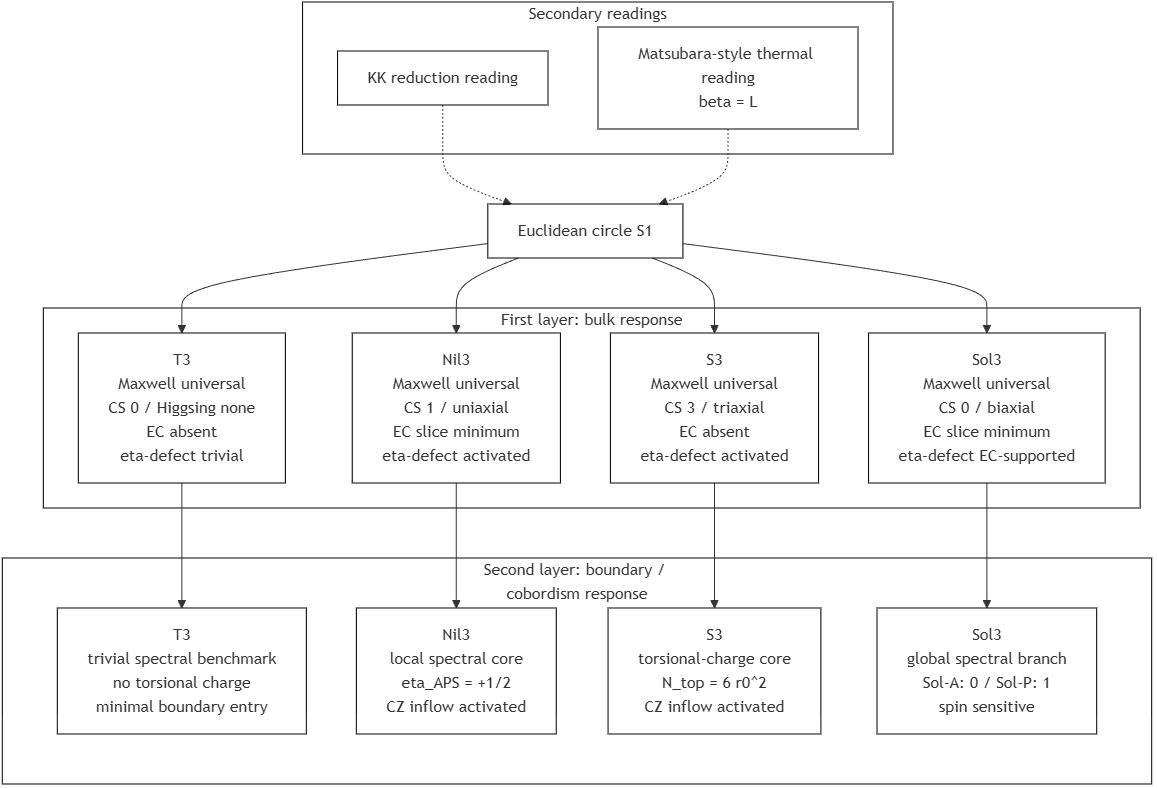
\includegraphics[width=0.95\linewidth]{figures/fig01_architecture_overview.png}
\caption{Two-layer architecture overview.  The first-layer bulk response and
the second-layer boundary/cobordism response are displayed along the four
geometries, while the KK reduction reading and the Matsubara-style thermal
reading---both arising from the same Euclidean circle---are separated as
secondary readings.}
\label{fig:architecture}
\end{figure}
   % Introduction
%==============================================================================
% Section 2: Homogeneous baseline
%==============================================================================
\section{Homogeneous Baseline}
\label{sec:baseline}

This section organises the homogeneous baseline of the four Thurston
geometries $\Tthree$, $\Nilthree$, $\Sthree$, $\Solthree$ and fixes the
comparison axis.  The aim is to align the mode language, the baseline
invariants, and the minimal/activated distinction of each geometry in a common
convention before the bulk/boundary response dictionaries of the subsequent
sections are introduced.  The selection rules that appear later are read off
from the baseline comparison fixed here.

\subsection{Four-Geometry Setup}
\label{sec:baseline:setup}

All four geometries compared in this paper share the common Euclidean product
structure $M^3\times\Sone$, but the structure constants of the
three-dimensional spatial part, the Weyl curvature, the KK splitting pattern,
and the frame rigidity differ from geometry to geometry.  Even with the same
minisuperspace variables, the stability of the effective potential, the mass
splitting of the vector sector, and the activation conditions of the
Chern--Simons channel therefore vary in a geometry-dependent way.

We first fix the homogeneous sector as a comparison baseline, on top of which
the first-layer bulk response and the second-layer boundary response are
stacked.  This makes the words \emph{activated}, \emph{protected}, and
\emph{minimal} read in subsequent sections not as descriptive labels but as
clear comparative judgements relative to the homogeneous background.

\subsection{Basic Comparison Table}
\label{sec:baseline:table}

The current baseline is summarised in the following table.

\begin{table}[H]
\centering
\begin{tabular}{lcccc}
\toprule
Indicator & $\Tthree$ & $\Nilthree$ & $\Sthree$ & $\Solthree$ \\
\midrule
CS direction count & 0 & 1 & 3 & 0 \\
KK Higgsing & none & uniaxial & triaxial & biaxial \\
EC slice minimum & absent & present & absent & present \\
Maxwell baseline & universal & universal & universal & universal \\
spin-2 rigidity & non-rigid & non-rigid & non-rigid & rigid \\
$C^2_\LC$ & $0$ & $4/(3R^4)$ & $0$ & $16/(3R^4)$ \\
\bottomrule
\end{tabular}
\caption{Four-geometry homogeneous baseline.}
\label{tab:baseline}
\end{table}

This table conveys two facts simultaneously.  First, $\Nilthree$ and $\Sthree$
are non-trivial activated geometries with respect to both the CS direction
count and the Higgsing pattern.  Second, $\Solthree$ is on the minimal side
in the CS direction count but possesses a non-vanishing Weyl curvature and
hence an EC slice-minimum branch isomorphic to that of $\Nilthree$.
Accordingly $\Solthree$ does not belong to the inert class of $\Tthree$; it is
a CS-inert but spin-0 active rigid geometry.  In the boundary layer this bulk
distinction is reinforced by the presence or absence of spectral branches
depending on the compact quotient and the spin structure.

\subsection{Maxwell Universality and the CS Direction-Count Law}
\label{sec:baseline:maxwell}

The first universal statement in the bulk layer is the geometry-independence
of the Maxwell coefficient.  Throughout this paper we adopt
\begin{equation}
  \KMxw = -\frac{L^2}{2r_0^4}
\end{equation}
as the baseline coefficient common to the four geometries.  This universality
keeps the skeleton of the main dictionary intact under inhomogeneous opening
and under either reading of the Euclidean circle.  Geometry dependence
therefore appears not in the Maxwell sector itself but in the CS-active
direction count, the Higgsing pattern, the EC slice-minimum structure, and
the defect response.

By contrast, Chern--Simons activation is geometry-dependent and the direction
count is set by the off-diagonal structure.  Activation occurs along one
direction in $\Nilthree$ and along three directions in $\Sthree$, while in
$\Solthree$ a self-referential cancellation forces it to zero.  The
distinction is decided not by ``whether structure constants exist'' but by
``whether the correction to $\tilde{F}_{ij}$ has its leg outside the index
pair $\{i,j\}$''.

The cancellation in $\Solthree$ arises because the underlying structure
constants form the symmetric pair
\begin{equation}
  C^1{}_{01} = +\frac{1}{R}, \qquad
  C^2{}_{02} = -\frac{1}{R},
\end{equation}
so that only same-leg self-coupling corrections remain.  Specifically the
correction $A_1\to\tilde{F}_{01}$ has its leg $1$ inside $\{0,1\}$ and is thus
self-referential, whereby the contributions $+1/R$ and $-1/R$ cancel
algebraically (off-diagonal CS rule, \S\ref{sec:rules:bulk} R2; details in
Appendix~\ref{app:E:E3}).  In this case the CS channel does not generate any
new parity-odd direction; only the biaxial Higgsing remains on top of the
Maxwell baseline.

\subsection{Mode Dictionary and Higgsing Pattern}
\label{sec:baseline:dict}

Read in the mode language, the differences among the four geometries in the
homogeneous sector concentrate in three sectors.  In the spin-0 sector, the
EC slice minimum on the $\eta=V=0$ section appears in $\Nilthree$ and
$\Solthree$.  Both share the same stationary radius and the same full
homogeneous Hessian criterion, but the slice potential and the radial Hessian
of $\Solthree$ are four times those of $\Nilthree$.  $\Tthree$ has a flat
zero slice and no isolated branch, while round $\Sthree$ has a non-zero
slope and no stationary point on the slice (verified in
Appendix~\ref{app:E:E5b}).  In the spin-1 sector the Higgsing pattern is
classified into none/uniaxial/triaxial/biaxial; this constitutes the principal
comparison axis of the bulk dictionary.  In the spin-2 sector only
$\Solthree$ exhibits frame rigidity; the other three geometries belong to the
non-rigid side.

In particular, the biaxial Higgsing of $\Solthree$ takes the form
\begin{equation}
  m^2(A_1) = m^2(A_2) = -\frac{L^2}{2r_0^4}, \qquad m^2(A_0) = 0.
\end{equation}
This follows from the modified field strength
$\tilde{F}_{01} = F_{01} + A_1/R$, which induces a mass term for $A_1$ and
$A_2$ with the same coefficient as $\KMxw$ (same-leg self-coupling), while
$A_0$ does not appear in $\tilde{F}$ and remains massless (KK derivation in
Appendix~\ref{app:E:E2}).  The fact that the two massive directions share the
same coefficient as the Maxwell baseline shows that $\Solthree$ is a distinct
geometry: it does not introduce a CS-active direction but carries an EC slice
branch and a rigid scaffold.

The four Higgsing types ``none/uniaxial/triaxial/biaxial'' are realised
exactly once each by $\Tthree, \Nilthree, \Sthree, \Solthree$, respectively,
as can be verified by direct computation of the KK mass matrices
(Appendix~\ref{app:E:E5}).

The role of this section is therefore to fix the baseline that supplies the
comparison axis of the response dictionary.  Most technical details---the
$\Solthree$ structure constants, the CS cancellation, and the frame
rigidity---are deferred to Appendices~\ref{app:A} and~\ref{app:E}.
   % Homogeneous baseline
%==============================================================================
% Section 3: Inhomogeneous / nonlocal bulk response
%==============================================================================
\section{Inhomogeneous / Nonlocal Bulk Response}
\label{sec:bulk}

This section treats the first-layer bulk response.  The aim is to fix, in the
form of an inventory and a set of selection rules, which response entries are
activated, protected, or absent for the four geometries once nonlocal /
inhomogeneous opening is allowed.  The bulk layer closes in a setting without
boundary, yet its internal structure already produces a sharp branching of
the response map across the four geometries.

\subsection{Definition of the Bulk Layer}
\label{sec:bulk:def}

By the first layer we mean the layer of responses that can be defined on the
bulk side without introducing a boundary.  In addition to the homogeneous
baseline---the Maxwell coefficient, the Chern--Simons direction count, and
the KK Higgsing pattern---it includes the presence/absence of an EC slice
minimum, the activation of parity-odd transport, the reduced $\eta$-mode
defect-localisation benchmark, and the opening pattern under inhomogeneous
perturbations.

The complete bulk inventory has a 36-entry structure (4 geometries
$\times$ 9 entries).  Rather than reproducing the full table in the body of
the paper, we present a compact summary table with the principal results and
a corresponding rule-set reading.  The full version is deferred to
Appendix~\ref{app:B}.

\subsection{Bulk Inventory: Overview}
\label{sec:bulk:inventory}

The principal bulk entries are as follows.

\begin{table}[H]
\centering
\resizebox{\linewidth}{!}{%
\begin{tabular}{lcccc}
\toprule
Entry & $\Tthree$ & $\Nilthree$ & $\Sthree$ & $\Solthree$ \\
\midrule
Maxwell coefficient & $-L^2/(2r_0^4)$ & $-L^2/(2r_0^4)$ & $-L^2/(2r_0^4)$ & $-L^2/(2r_0^4)$ \\
CS direction count & 0 & 1 & 3 & 0 \\
KK Higgsing type & none & uniaxial & triaxial & biaxial \\
EC slice minimum & absent & present & absent & present \\
$P$-linear transport & protected & activated & activated & protected \\
spin-2 rigidity & non-rigid & non-rigid & non-rigid & rigid \\
nonlinear opening & absent & absent & activated & absent \\
defect-localisation response ($\eta$ benchmark) & trivial & activated & activated & EC-supported / CS-inert \\
inhomogeneous bulk response & trivial & activated & activated & CS-inert / EC-active \\
\bottomrule
\end{tabular}%
}
\caption{Compact bulk inventory across the four geometries.}
\label{tab:bulk}
\end{table}

This table makes explicit that the first principal result of the paper lies
precisely in the activation map of the bulk layer.  While the Maxwell
coefficient is fully universal, the CS direction count, Higgsing type, EC
slice minimum, and defect-benchmark response differ from geometry to
geometry: the essence of the bulk layer lies less in coefficient differences
than in the differences in the type of allowed responses.

Read as rules, the inventory positions $\Nilthree$ as the geometry where CS
and the EC slice minimum simultaneously rise, $\Sthree$ as the most richly
CS- and Higgsing-activated geometry, $\Tthree$ as an inert benchmark, and
$\Solthree$ as a CS-inert geometry that nevertheless carries an EC slice
minimum and a rigid scaffold.

\subsection{Universal Channel and Activated Channel}
\label{sec:bulk:universal}

The most important bulk-layer formula is the Maxwell baseline common to all
four geometries:
\begin{equation}
  \KMxw^{\Tthree}
  = \KMxw^{\Nilthree}
  = \KMxw^{\Sthree}
  = \KMxw^{\Solthree}
  = -\frac{L^2}{2r_0^4}.
\end{equation}
This universal formula provides a reference plane that aligns the four
geometries onto a common dictionary.  Geometry-dependent differences appear
in the Chern--Simons activation rule and in the Higgsing classification.  In
$\Nilthree$ a single off-diagonal active direction emerges, while in
$\Sthree$ all three directions are activated equivalently.  By contrast in
$\Solthree$ the self-referential corrections cancel, so that
\begin{equation}
  \mathrm{CS}(R) = 0
  \qquad \Longrightarrow \qquad
  \delta_{\mathrm{CS}} = 0,\ \delta P = 0
\end{equation}
holds algebraically.

In this sense $\Solthree$ is not a CS-active geometry.  Unlike $\Tthree$,
however, $\Solthree$ carries a biaxial KK splitting, frame rigidity, and an
EC slice-minimum branch, so it is not a complete inert benchmark even at the
bulk layer.  In the boundary layer the possibility of a spectral branch
depending on the compact quotient and the spin structure remains, so its
CS-inertness should not be lifted directly to triviality at the second layer.

The mechanism behind this difference is geometry-specific.  In $\Solthree$
the symmetric pair of structure constants
\begin{equation}
  C^1{}_{01} = +\frac{1}{R}, \qquad
  C^2{}_{02} = -\frac{1}{R}
\end{equation}
ensures that the non-abelian cubic correction does not increase the
parity-odd channel count.  Specifically, the legs of both corrections
$A_1\to\tilde{F}_{01}$ and $A_2\to\tilde{F}_{02}$ lie \emph{inside} the index
pairs $\{0,1\}$ and $\{0,2\}$ respectively, so that no off-diagonal CS
direction is generated for any profile-local scalar coefficients
$c_{01}, c_{02}$ (off-diagonal CS rule; see
Appendices~\ref{app:E:E3} and~\ref{app:E:E4}).  In $\Nilthree$, on the other
hand, a non-trivial structure constant exists in only one direction; this
uniaxiality is the origin of both the one-direction CS activation and the
EC slice-minimum branch.  In $\Sthree$ the isotropic coupling structure
preserves a three-fold degeneracy and admits a nonlinear opening through
higher-order couplings.

\begin{figure}[H]
\centering
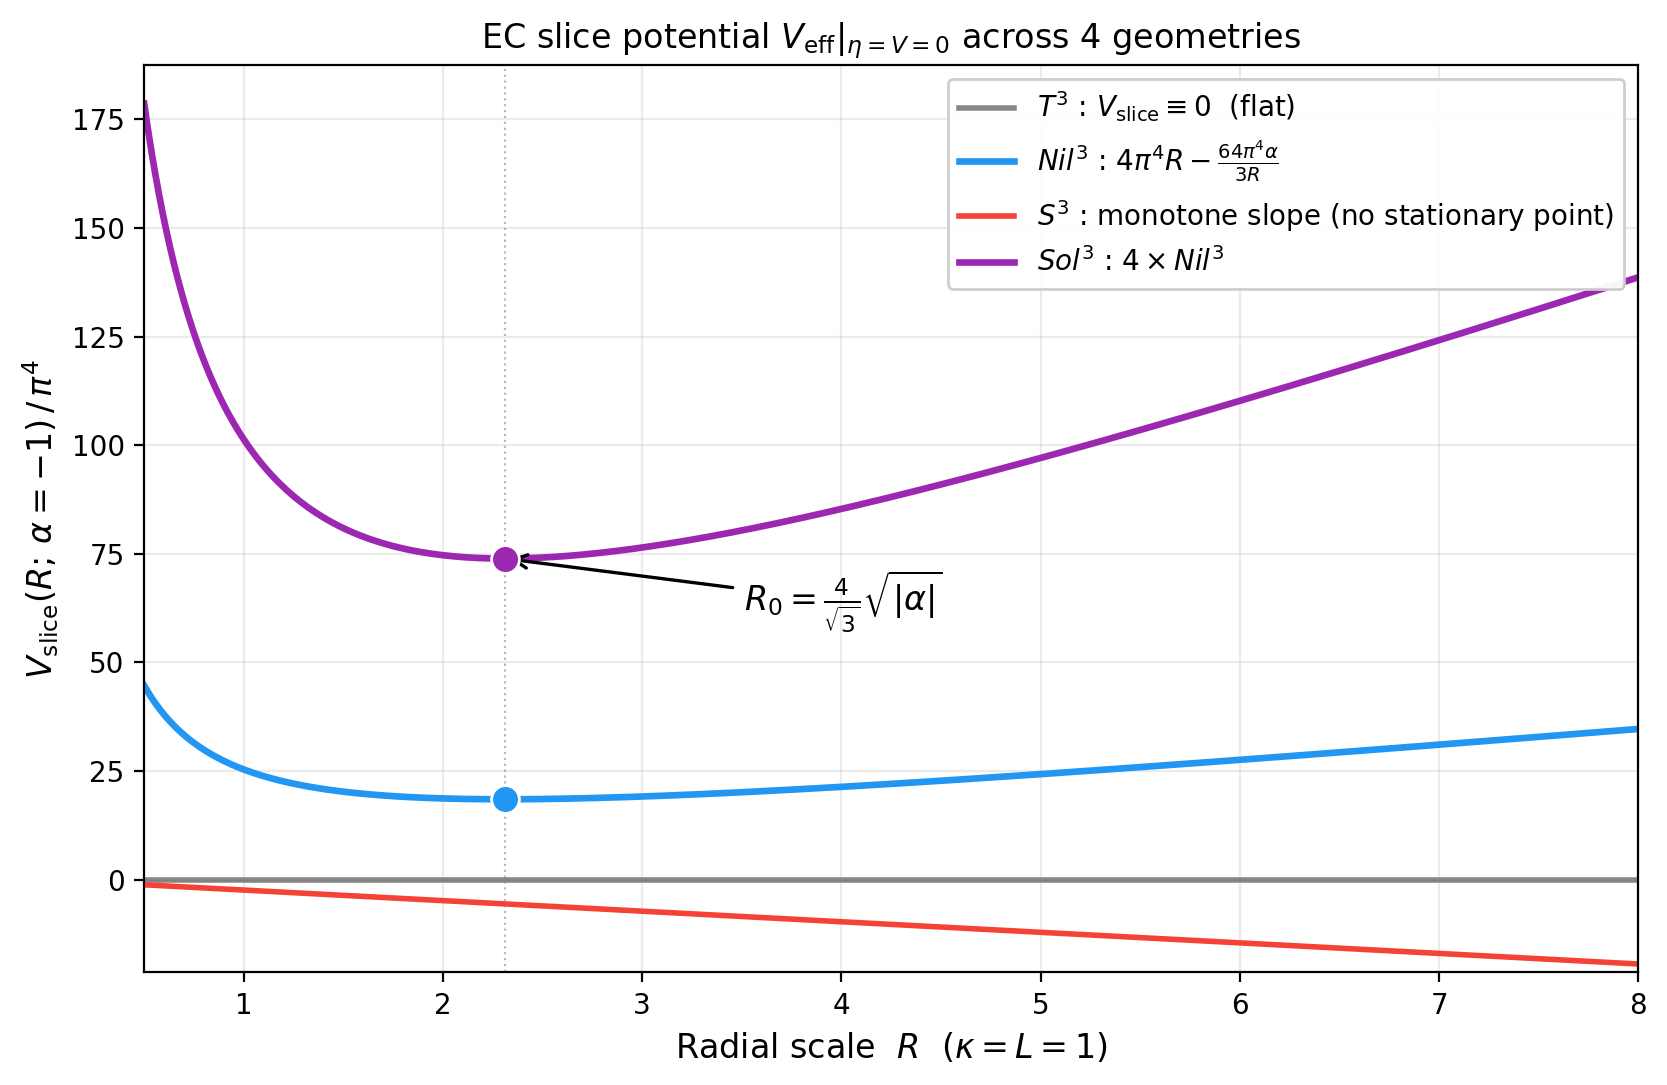
\includegraphics[width=0.85\linewidth]{figures/fig02_ec_slice_potential.png}
\caption{Comparison of the EC slice potential $\Veff(\eta=V=0,R)$ across the
four geometries.  In $\Nilthree$ and $\Solthree$ a stationary branch
appears, with the slice potential of $\Solthree$ being four times that of
$\Nilthree$.  $\Tthree$ has a flat zero slice and round $\Sthree$ has a
non-zero slope without a stationary point.}
\label{fig:ec_slice}
\end{figure}

\subsection{Reduced $\eta$-Mode Defect-Localisation Benchmark}
\label{sec:bulk:defect}

To compare the four geometries on equal footing when an inward radial dip or
localised defect is opened, we adopt the reduced 1D AX-torsion ansatz
\begin{equation}
  \eta = \eta(z)
\end{equation}
on a slice-wise homogeneous background.  Setting the radial scale as
\begin{equation}
  \rho(z) = r(z) \quad (\Tthree, \Sthree),
  \qquad
  \rho(z) = R(z) \quad (\Nilthree, \Solthree),
\end{equation}
the localisation benchmark operator reduces to the Sturm--Liouville form
\begin{equation}
  -\frac{\dd}{\dd z}\!\left[K_{\mathrm{geo}}(z)\frac{\dd f}{\dd z}\right]
  + M_{\mathrm{geo}}(z) f = E f,
  \qquad
  K_{\mathrm{geo}}(z) = M_{\mathrm{geo}}(z) = c_{\mathrm{geo}}\,\rho(z).
\end{equation}
The coefficient $c_{\mathrm{geo}}$ is topology-dependent:
\begin{equation}
  c_{\Tthree} = c_{\Nilthree} = c_{\Solthree} = \frac{96\pi^4 L}{\kappa^2},
  \qquad
  c_{\Sthree} = \frac{12\pi^2 L}{\kappa^2}.
\end{equation}
Here $M_{\mathrm{geo}}$ is the exact homogeneous datum
\begin{equation}
  M_{\mathrm{geo}} = \left.\frac{\partial^2 \Veff}{\partial \eta^2}\right|_{\eta=0}
\end{equation}
obtained from the current \texttt{dppu} library, and $K_{\mathrm{geo}}$ is the
reduced 1D datum coming from the AX contortion gradient; the agreement of the
two is verified in Appendix~\ref{app:E:E6}.

For a Gaussian $\rho$-dip
\begin{equation}
  \rho(z) = \rho_0\bigl(1 - A\,e^{-z^2/w^2}\bigr), \qquad 0 < A < 1,
\end{equation}
a variational evaluation with the trial function $f_\lambda = e^{-\lambda |z|}$
yields $E_{\mathrm{var}}(\lambda) < M_0 = c_{\mathrm{geo}}\rho_0$ for
sufficiently small $\lambda > 0$, so that the existence of at least one bound
state is established analytically (Appendix~\ref{app:E:E6}).  Localisation
itself therefore holds at the level of this reduced benchmark for all four
geometries.  Representative numerical scans corroborate this: $E_{\min}<M_0$
holds across all $4\times 3 = 12$ examples (4 geometries $\times$ 3 Gaussian
$\rho$-dip profiles); see scripts \texttt{paper04/eta\_defect\_coefficients.py}
and \texttt{paper04/defect\_localization.py}.

\begin{figure}[H]
\centering
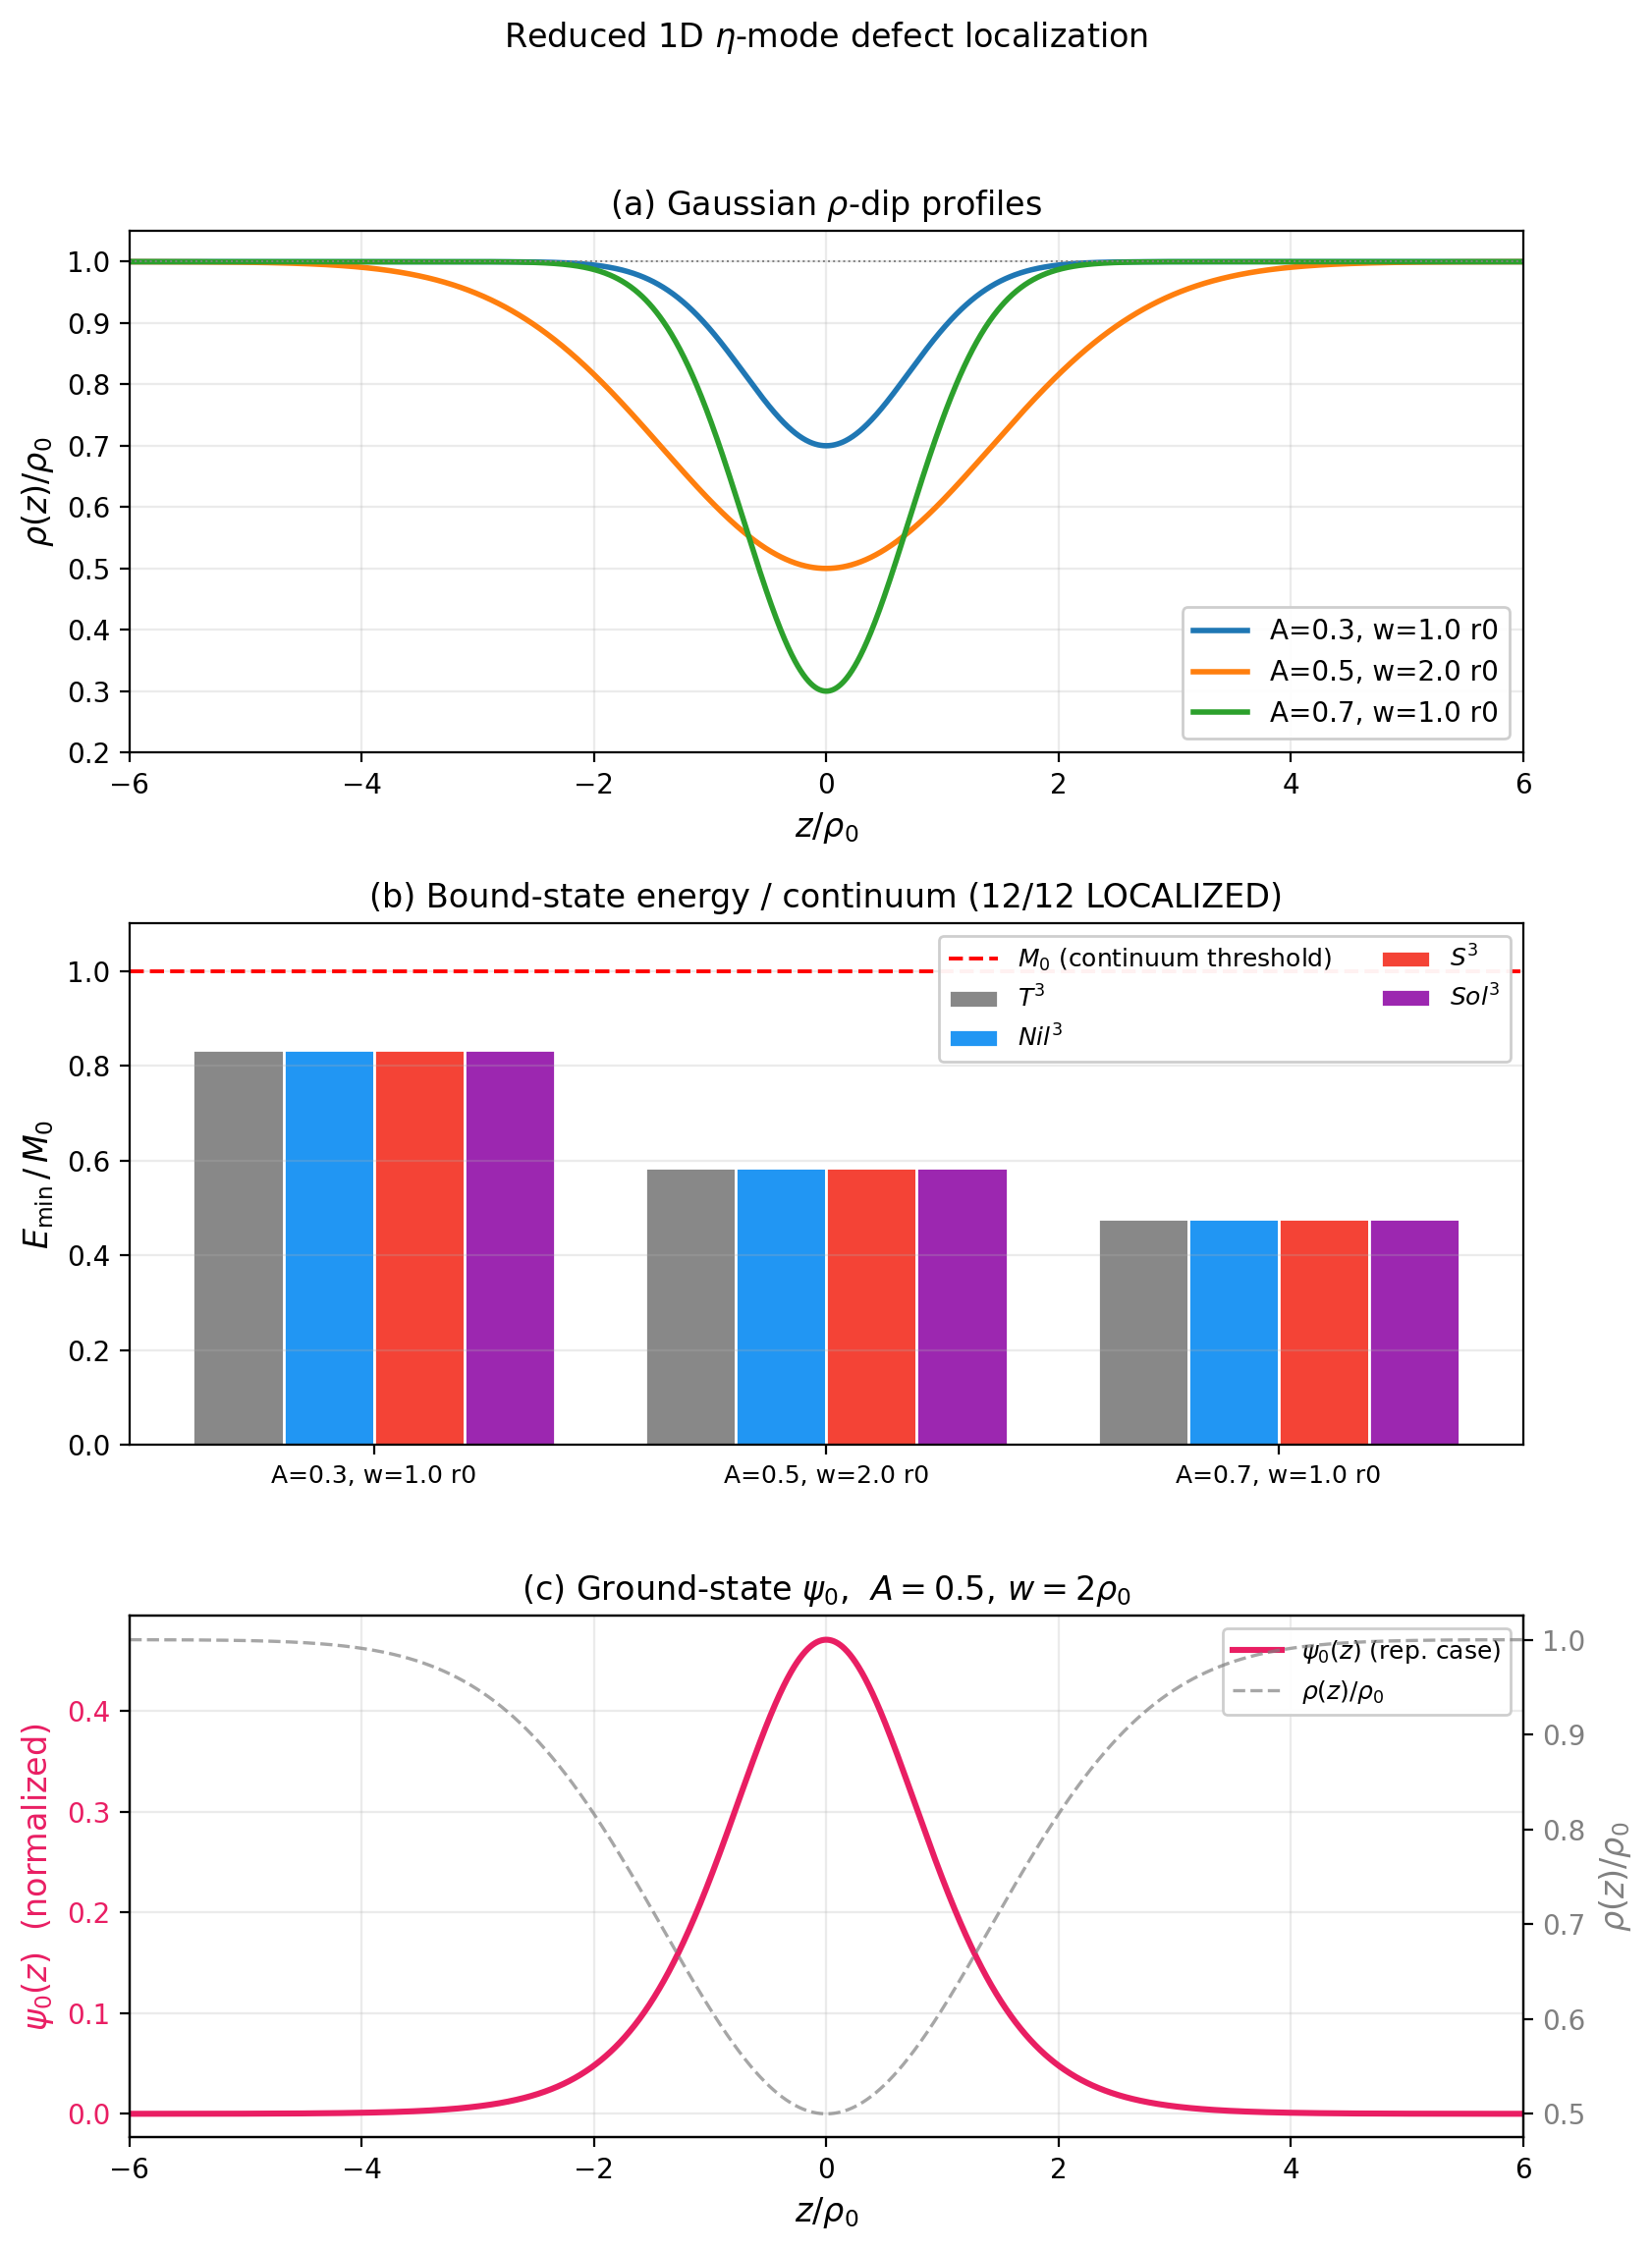
\includegraphics[width=0.85\linewidth]{figures/fig03_defect_localization.png}
\caption{Reduced $\eta$-mode defect-localisation benchmark.  The Gaussian
$\rho$-dip, the effective potential $M_{\mathrm{geo}}(z)$, the bound-state
energy $E_{\min} < M_0$, and the ground-state wavefunction are displayed
within the same 1D benchmark.  Localisation itself is common to the four
geometries; differences in activation are determined by the subsequent
CS / EC / nonlinear structure.}
\label{fig:defect}
\end{figure}

In $\Tthree$ this common benchmark stays on the kinematic / trivial side.  In
$\Solthree$ the EC slice minimum is present so that the spin-0 sector is
active, but the CS direction count remains zero so that the response does
not progress to torsional-charge or local parity-odd activation.  In
$\Nilthree$, by contrast, the EC slice minimum and the CS-active structure
combine so that the localised $\eta$-mode is tied to the activation of the
spectral / parity-odd channel.  In $\Sthree$ the triplet degeneracy and the
nonlinear opening overlap, producing the richest activation pattern.  Hence
the labels ``trivial / activated'' in the row record not the existence of a
bound state \emph{per se}, but how the common reduced $\eta$-benchmark
combines with the additional bulk structure.

\subsection{Geometry-Wise Bulk Reading}
\label{sec:bulk:reading}

The bulk-layer reading splits across the four geometries as follows.

\begin{itemize}
  \item $\Tthree$: flat and inert.  The response is minimal and many bulk
        entries are trivial / protected.  It serves as the reference geometry
        for the comparison dictionary.
  \item $\Nilthree$: the first activated geometry.  It carries CS-active
        structure, an EC slice minimum, and a uniaxial Higgsing, and connects
        naturally to the strict APS spectral core appearing on the boundary.
  \item $\Sthree$: the richest activated geometry.  It exhibits isotropic
        degeneracy, an activated parity-odd channel, and a nonlinear opening,
        and yields a frame-bundle-normalised torsional-charge core on the
        boundary.
  \item $\Solthree$: a distinct geometry that is CS-inert yet carries an EC
        slice minimum, a biaxial KK splitting, and frame rigidity.  In the
        boundary layer it can support a global spectral branch depending on
        the compact quotient and the spin structure.
\end{itemize}

\subsection{Summary}
\label{sec:bulk:summary}

The significance of the bulk layer is that it closes the response inventory
of the four geometries in the form of first-layer selection rules.  The
organisation obtained here is reused, in the subsequent boundary/cobordism
layer, as the comparison axis for deciding ``which channel is non-trivial in
which geometry''.
   % Inhomogeneous / nonlocal bulk response
%==============================================================================
% Section 4: Boundary / interface response
%==============================================================================
\section{Boundary / Interface Response}
\label{sec:boundary}

This section addresses the second-layer boundary/cobordism response.  We
present the geometry-wise inventory, the observable taxonomy, the pairwise
cobordism dictionary, and the geometric scaffold layer as a single structure.
While the bulk layer is mainly concerned with ``what each geometry allows in
isolation,'' the second layer makes explicit ``what survives as an observable
on the boundary'' and ``which observables make geometry pairs comparable''.

\subsection{CZ Inflow and Notation}
\label{sec:boundary:cz}

In the second layer at least three different 3-forms must be carefully
distinguished:
\begin{itemize}
  \item $\Ctor$: torsion-CS 3-form,
  \item $\Csig$: spinor CS 3-form,
  \item $\Cadj$: adjoint CS 3-form.
\end{itemize}
We write the Chandia--Zanelli inflow \cite{Chandia1997} as
\begin{equation}
  \SCZ[M_3] = \frac{k_{\mathrm{cl}}}{4\pi^2}\int_{M_3} \Ctor.
\end{equation}
The relation
\begin{equation}
  \mathrm{NY} = \dd \Ctor,
  \qquad
  \dd \Ctor = T^a\wedge T_a + R_{ab}\wedge e^a\wedge e^b
\end{equation}
between the Nieh--Yan density and $\Ctor$ then connects the boundary inflow
directly to NY.  By contrast the APS spectral entry \cite{APS1975} is
defined via $\Csig = \Tr_\sigma(\omega\wedge \dd\omega + \tfrac{2}{3}\omega^3)$,
constructed only from the Levi--Civita connection; the two forms must not
be conflated.  The adjoint CS 3-form $\Cadj$ appears at intermediate stages
of the APS argument but is not the final spectral observable itself
(Appendix~\ref{app:E:E8}).

This distinction is essential for the taxonomy that follows.  The strict APS
entry of $\Nilthree$ and the frame-bundle-normalised torsional-charge entry
of $\Sthree$ are both parity-odd boundary quantities, but they belong to
different families.  Even within the spectral family, moreover, the source is
not uniform: the strict value of $\Nilthree$ is a local spectral core
provided by a non-zero Levi--Civita spinor CS integral, whereas the APS
branch on the compact $\Solthree$ benchmark is a global spectral branch
that arises from kernel/spin-structure data while the local CS integral
itself vanishes.

\subsection{Geometry-Wise Boundary Inventory}
\label{sec:boundary:inventory}

The geometry-wise boundary inventory is summarised as follows.

\begin{table}[H]
\centering
\resizebox{\linewidth}{!}{%
\begin{tabular}{lcccc}
\toprule
Entry & $\Tthree$ & $\Nilthree$ & $\Sthree$ & $\Solthree$ \\
\midrule
CS interface jump & absent & present & present & absent \\
APS $\eta$-invariant & $0$ & strict $+1/2$ (local) & $0$ & $0/1$ (Sol-A / Sol-P) \\
CZ inflow & absent & activated & activated & absent \\
edge / interface mode & minimal & activated & activated & spin-sensitive \\
boundary tag & trivial benchmark & APS local core & torsional-charge active & global spectral branch \\
\bottomrule
\end{tabular}%
}
\caption{Geometry-wise boundary inventory.}
\label{tab:boundary}
\end{table}

The principal entry of $\Nilthree$ is the strict APS spectral core, with
canonical value
\begin{equation}
  \etaAPS(\Nilthree) = +\frac{1}{2}.
\end{equation}
The Heisenberg mode decomposition shows that, with PPA spin structure, the
condition $p_2\in\mathbb{Z}+1/2$ excludes the $p_2 = 0$ zero mode, so that the
$n=0$ spin-up branch alone carries the spectral asymmetry.  The value itself
is obtained from the Levi--Civita spinor Chern--Simons integral of $\Nilthree$,
\begin{equation}
  \int_Y \Csig = -\frac{1}{2},
\end{equation}
combined with the DPPU orientation convention
$\etaAPS = -\int_Y \Csig$, giving
\begin{equation}
  \etaAPS = +\frac{1}{2}, \qquad \eta(0) = 2\etaAPS - h = 1
\end{equation}
(Appendix~\ref{app:E:E10}; verification: \texttt{paper04/eta\_aps\_nil3.py}).
Crucially, this spectral value originates from Levi--Civita spinor spectral
data rather than from the torsion-CS sector.  Although $\Nilthree$ also
carries CZ inflow, the strict core that takes precedence is the spectral
family, and its source is local.  As benchmarks, the PPA spin structure on
$\Tthree$ and the Levi--Civita Dirac on round $\Sthree$ both have spectra
exactly symmetric under $\lambda\leftrightarrow -\lambda$, giving
$\etaAPS = 0$ (verification: \texttt{proofs/aps\_zero\_t3\_s3.py}).

\begin{figure}[H]
\centering
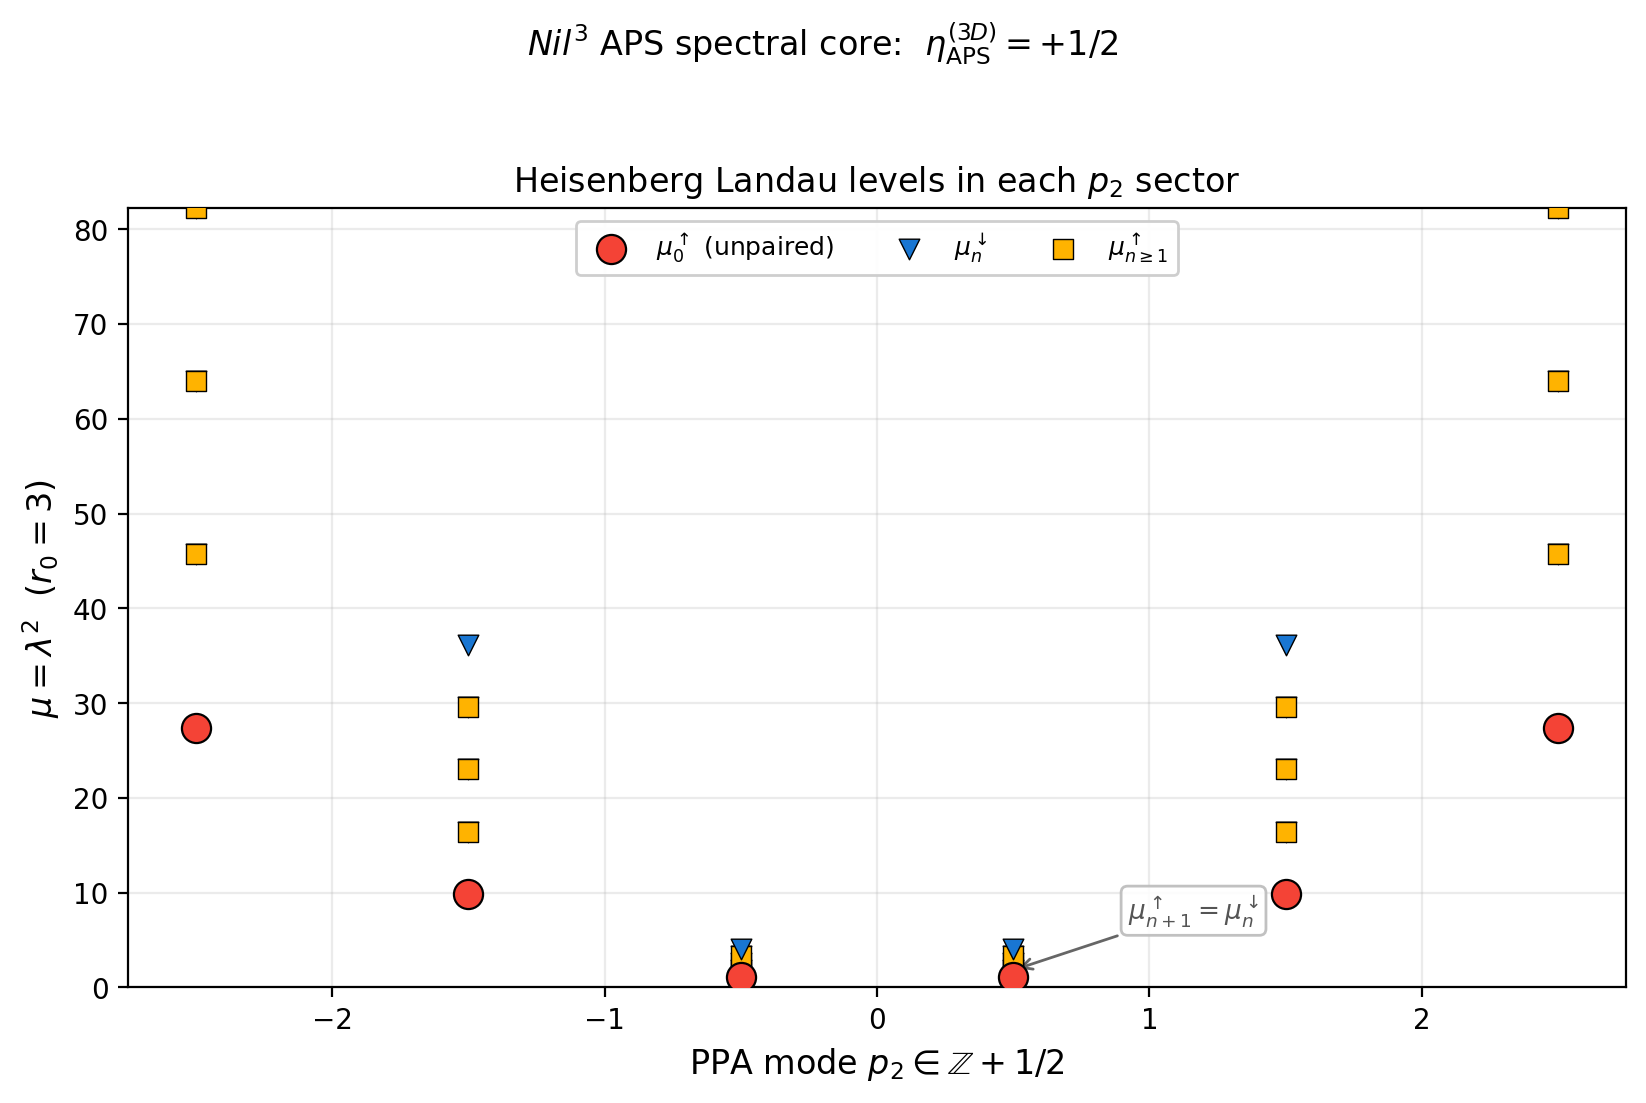
\includegraphics[width=0.85\linewidth]{figures/fig04_nil3_aps.png}
\caption{$\Nilthree$ Heisenberg Landau-level spectrum and the construction of
$\etaAPS$.  Under the PPA spin structure the $n=0$ spin-up branch carries
the spectral asymmetry, and the Levi--Civita spinor CS integral gives
$\etaAPS(\Nilthree) = +1/2$.}
\label{fig:nil3_aps}
\end{figure}

For $\Solthree$ the situation is different.  Taking the compact mapping-torus
benchmark
\begin{equation}
  M_A = T^2\rtimes_A \Sone,
  \qquad
  A = \begin{pmatrix}2 & 1 \\ 1 & 1\end{pmatrix},
\end{equation}
together with the two spin structures Sol-P and Sol-A tracked within DPPU,
the local Levi--Civita Chern--Simons integral itself vanishes:
\begin{equation}
  \int_Y \Csig = 0.
\end{equation}
Here ``Sol-P'' denotes the benchmark with periodic base circle and periodic
fibre, and ``Sol-A'' the benchmark with anti-periodic base circle and
periodic fibre.  The Dirac kernel branches as
\begin{equation}
  h(\text{Sol-P}) = 2, \qquad h(\text{Sol-A}) = 0,
\end{equation}
and the antilinear time-reversal symmetry gives $\eta(0) = 0$, so that
\begin{equation}
  \etaAPS(\text{Sol-P}) = 1, \qquad
  \etaAPS(\text{Sol-A}) = 0
\end{equation}
(Appendix~\ref{app:E:E10b}; verification: \texttt{proofs/eta\_aps\_sol3.py}).
$\Solthree$ is therefore not a ``local APS core'' but a global spectral
branch that switches on/off according to the compact quotient and the spin
structure.

\begin{figure}[H]
\centering
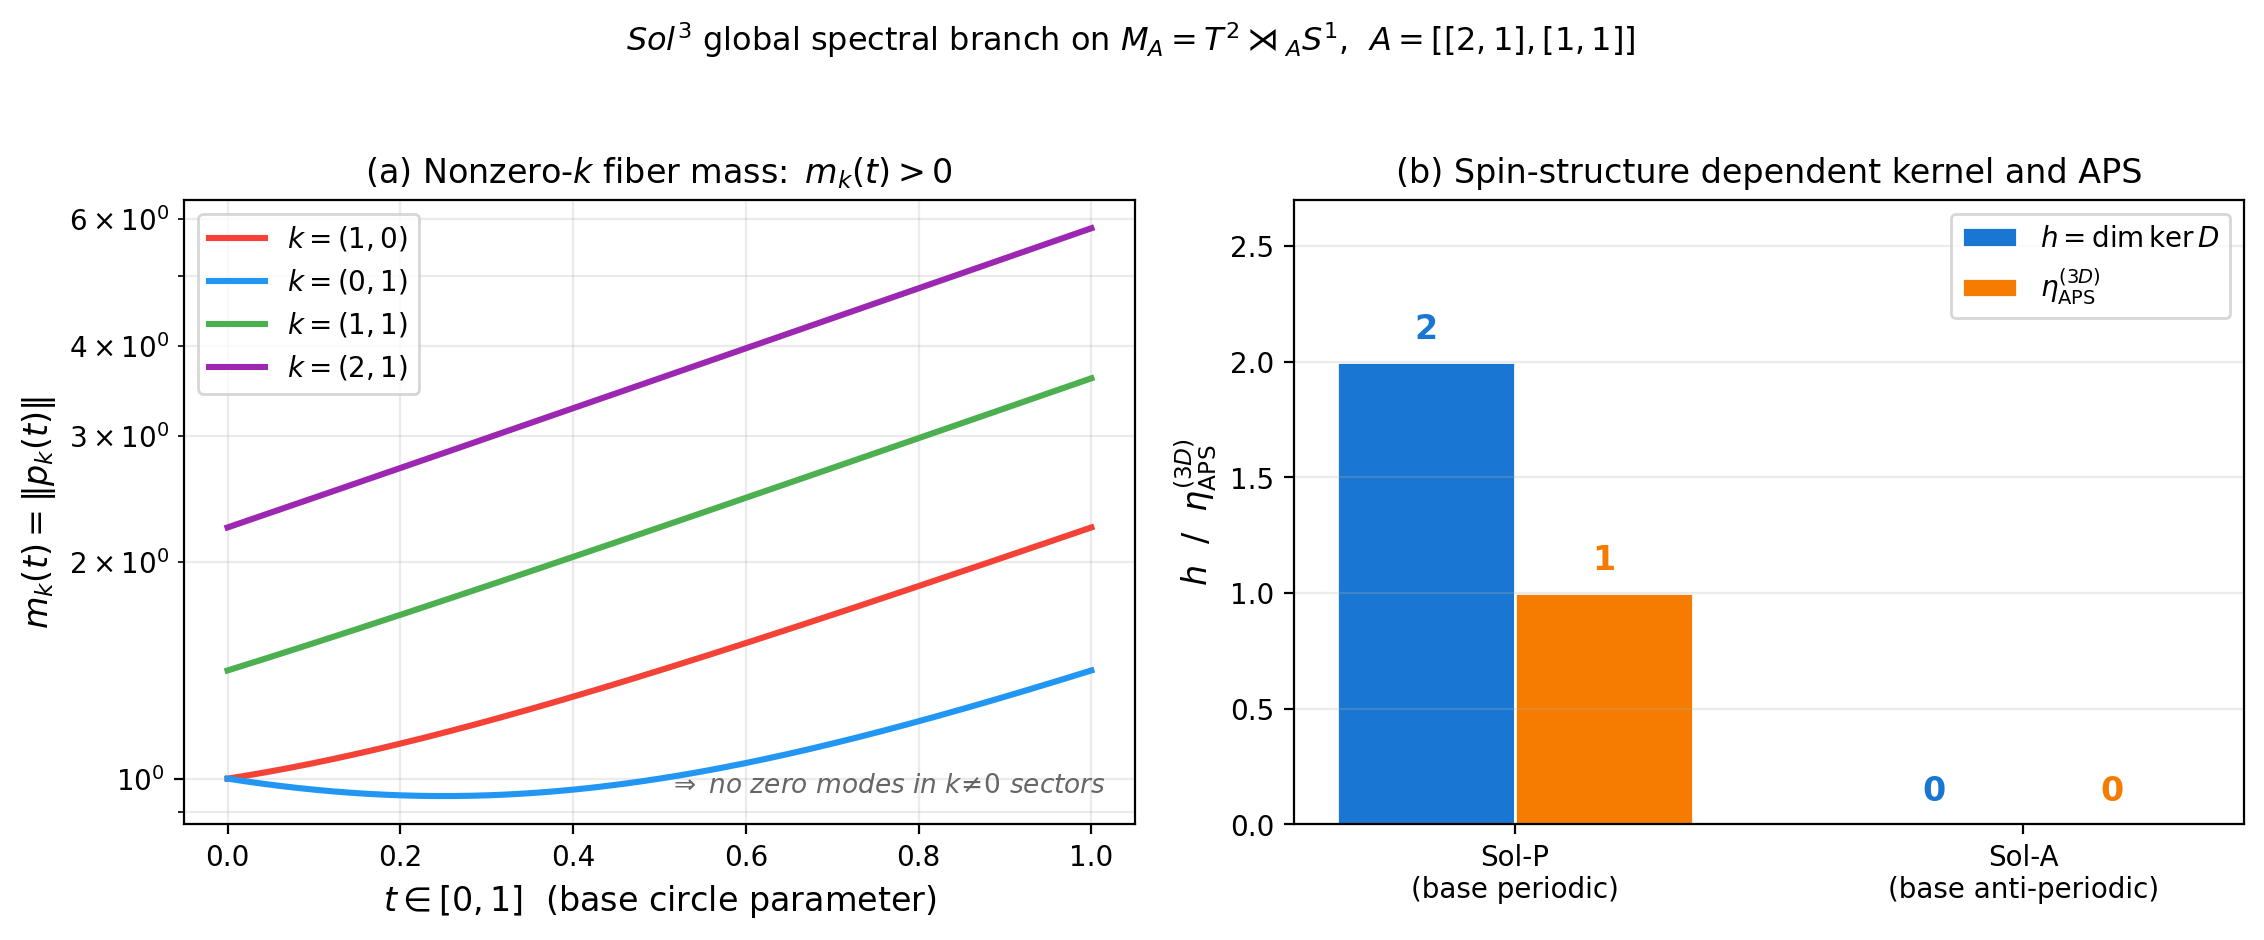
\includegraphics[width=0.85\linewidth]{figures/fig05_sol3_global_spectral.png}
\caption{Global spectral branch of $\Solthree$.  On the compact mapping-torus
benchmark the kernel dimension $h$ and $\etaAPS$ branch between Sol-P and
Sol-A; the on/off switching is driven by global / spin-structure data
rather than by the local CS integral.}
\label{fig:sol3_global}
\end{figure}

The principal entry of $\Sthree$ is the frame-bundle-normalised
torsional-charge core characterised by
\begin{equation}
  \Ntop = 6 r_0^2.
\end{equation}
The geometric part follows from the structure constants
$C^i{}_{jk} = (4/r_0)\,\epsilon^i{}_{jk}$ via
$T^i = \tfrac{1}{2}C^i{}_{jk}\,e^j\wedge e^k$ and
\begin{equation}
  \Ctor = e_i\wedge T^i = \frac{12}{r_0}\,\mathrm{vol}_{\Sthree}
  \quad\Longrightarrow\quad
  \int_{\Sthree}\Ctor = 24\pi^2 r_0^2.
\end{equation}
The factor $1/(4\pi^2)$ is the frame-bundle normalisation associated with
$\pi_3(SO(3)) = \mathbb{Z}$ ($T_R = 1$), leading to $\Ntop = 6 r_0^2$
(Appendix~\ref{app:E:E9}).  Since no extra quantisation condition on $r_0$
is imposed, $\Ntop$ here is the frame-bundle-normalised torsional charge.
The interface CS jump and the CZ inflow belong to this torsional sector and
underpin the role of $\Sthree$ in the pairwise dictionary as the
torsional-charge-led geometry.

$\Tthree$ has all boundary entries trivial and serves as a benchmark.  Yet
$\Solthree$ is CS-inert while still carrying an EC slice minimum and a rigid
scaffold; in the boundary layer it can support a global spectral branch
depending on the compact quotient and the spin structure.  Collapsing
$\Tthree$ and $\Solthree$ into a single second-layer class is therefore
inaccurate.  Independently of the presence/absence of a boundary spectral
branch, the fact that $\Solthree$ has a distinct, non-flat background
geometry is preserved.

\subsection{Observable Taxonomy}
\label{sec:boundary:taxonomy}

We classify the second-layer observables into the following three families.

\begin{table}[H]
\centering
\resizebox{\linewidth}{!}{%
\begin{tabular}{llllc}
\toprule
Family & Representative & Carrier & Value type & Canonical geometry \\
\midrule
spectral & $\etaAPS$ & LC spectral data ($\Csig$ and/or kernel/spin) & half-int. / int.\ branch & $\Nilthree$ (local), $\Solthree$ (global) \\
torsional-charge & $\Ntop$ & frame-bundle normalisation of $\Ctor$ & frame-bundle-norm.\ torsional charge & $\Sthree$ \\
inflow & $\SCZ$ & $\Ctor$ & boundary functional & $\Nilthree$, $\Sthree$ \\
\bottomrule
\end{tabular}%
}
\caption{Three observable families of the second layer.}
\label{tab:taxonomy}
\end{table}

These three families furnish the observable taxonomy of the second layer.
The crucial point is that, although $\etaAPS$ and $\Ntop$ are both
non-trivial boundary quantities, they are not of the same type and should
not be subtracted directly.  Quantities universally comparable in pairwise
comparison reside instead on the side of the inflow functional written in
terms of $\Ctor$.

\subsection{Pairwise Cobordism Dictionary}
\label{sec:boundary:pairwise}

Six pairs are obtained from the four geometries.  We summarise the dominant
observable and source relation for each pair.

\begin{table}[H]
\centering
\resizebox{\linewidth}{!}{%
\begin{tabular}{lcll}
\toprule
Pair & Class & Dominant observable & Note \\
\midrule
$\Sthree \leftrightarrow \Tthree$ & torsional / trivial & frame-bundle-norm.\ torsional charge & $\Sthree$ benchmark \\
$\Sthree \leftrightarrow \Nilthree$ & torsional / local spectral & mixed & torsional-charge crosses local spectral \\
$\Sthree \leftrightarrow \Solthree$ & torsional / global spectral & spin-sensitive & torsional-led for Sol-A; mixed for Sol-P \\
$\Tthree \leftrightarrow \Nilthree$ & trivial / local spectral & spectral & $\Nilthree$ local core dominates \\
$\Tthree \leftrightarrow \Solthree$ & trivial / global spectral & spin-sensitive & Sol-A: trivial; Sol-P: global spectral \\
$\Nilthree \leftrightarrow \Solthree$ & local / global spectral & spectral & source comparison within spectral family \\
\bottomrule
\end{tabular}%
}
\caption{Pairwise cobordism dictionary.}
\label{tab:pairwise}
\end{table}

\begin{figure}[H]
\centering
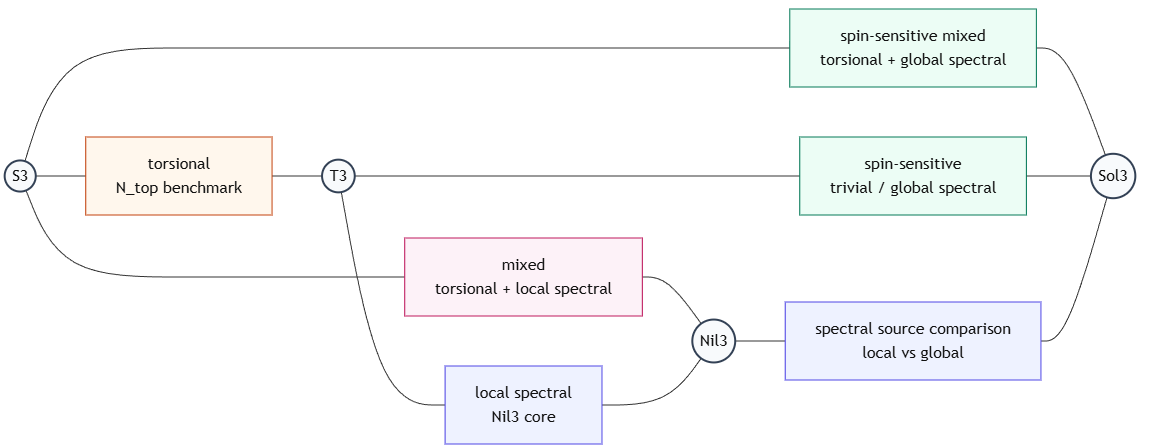
\includegraphics[width=0.9\linewidth]{figures/fig06_pairwise_cobordism_dictionary.png}
\caption{Pairwise cobordism dictionary.  The four geometries form the
vertices of a pair graph; the six pairs are labelled with the dominant
observable and the spin-sensitivity.  Pairs containing $\Sthree$ tend to be
torsional-charge-led, whereas pairs containing $\Solthree$ admit a global
spectral branch governed by the compact quotient and the spin structure.}
\label{fig:pairwise}
\end{figure}

This table captures the comparison logic of the paper most directly: the
geometry-wise inventory translated into the language of pairwise cobordism.
In particular, $\Sthree\leftrightarrow\Nilthree$ is the intersection of the
torsional-charge family and the local spectral family, while
$\Nilthree\leftrightarrow\Solthree$ encodes a ``local vs.\ global'' source
distinction within the spectral family itself.  $\Tthree\leftrightarrow\Solthree$
is not a uniformly inert pair either: it overlaps the trivial benchmark for
Sol-A, while a global spectral branch arises for Sol-P, making it a
spin-sensitive pair.

The advantage of the pairwise dictionary is that it makes simultaneously
explicit ``which observable family is the subject of comparison'' and
``whether the value is local or global''---features hard to read off from a
geometry-by-geometry inventory alone.  The tendency that pairs containing
$\Sthree$ are torsional-charge-led, those containing $\Nilthree$ are
local-spectral-led, and those containing $\Solthree$ may carry a global
spectral branch depending on the compact quotient and spin structure
underpins the concise statement of the selection rules.

\subsection{Geometric Scaffold Layer}
\label{sec:boundary:scaffold}

While not an observable family, we also record the following scaffold-layer
quantities, which characterise the background geometry.

\begin{table}[H]
\centering
\begin{tabular}{lccc}
\toprule
Geometry & $C^2_\LC$ & spin-2 rigidity tag & $\AKK / K^2$ \\
\midrule
$\Tthree$ & $0$ & trivial & $0$ \\
$\Nilthree$ & $4/(3R^4)$ & non-rigid & $2/3$ \\
$\Sthree$ & $0$ & non-rigid & $0$ \\
$\Solthree$ & $16/(3R^4)$ & rigid & $2/3$ \\
\bottomrule
\end{tabular}
\caption{Geometric scaffold quantities.}
\label{tab:scaffold}
\end{table}

\begin{figure}[H]
\centering
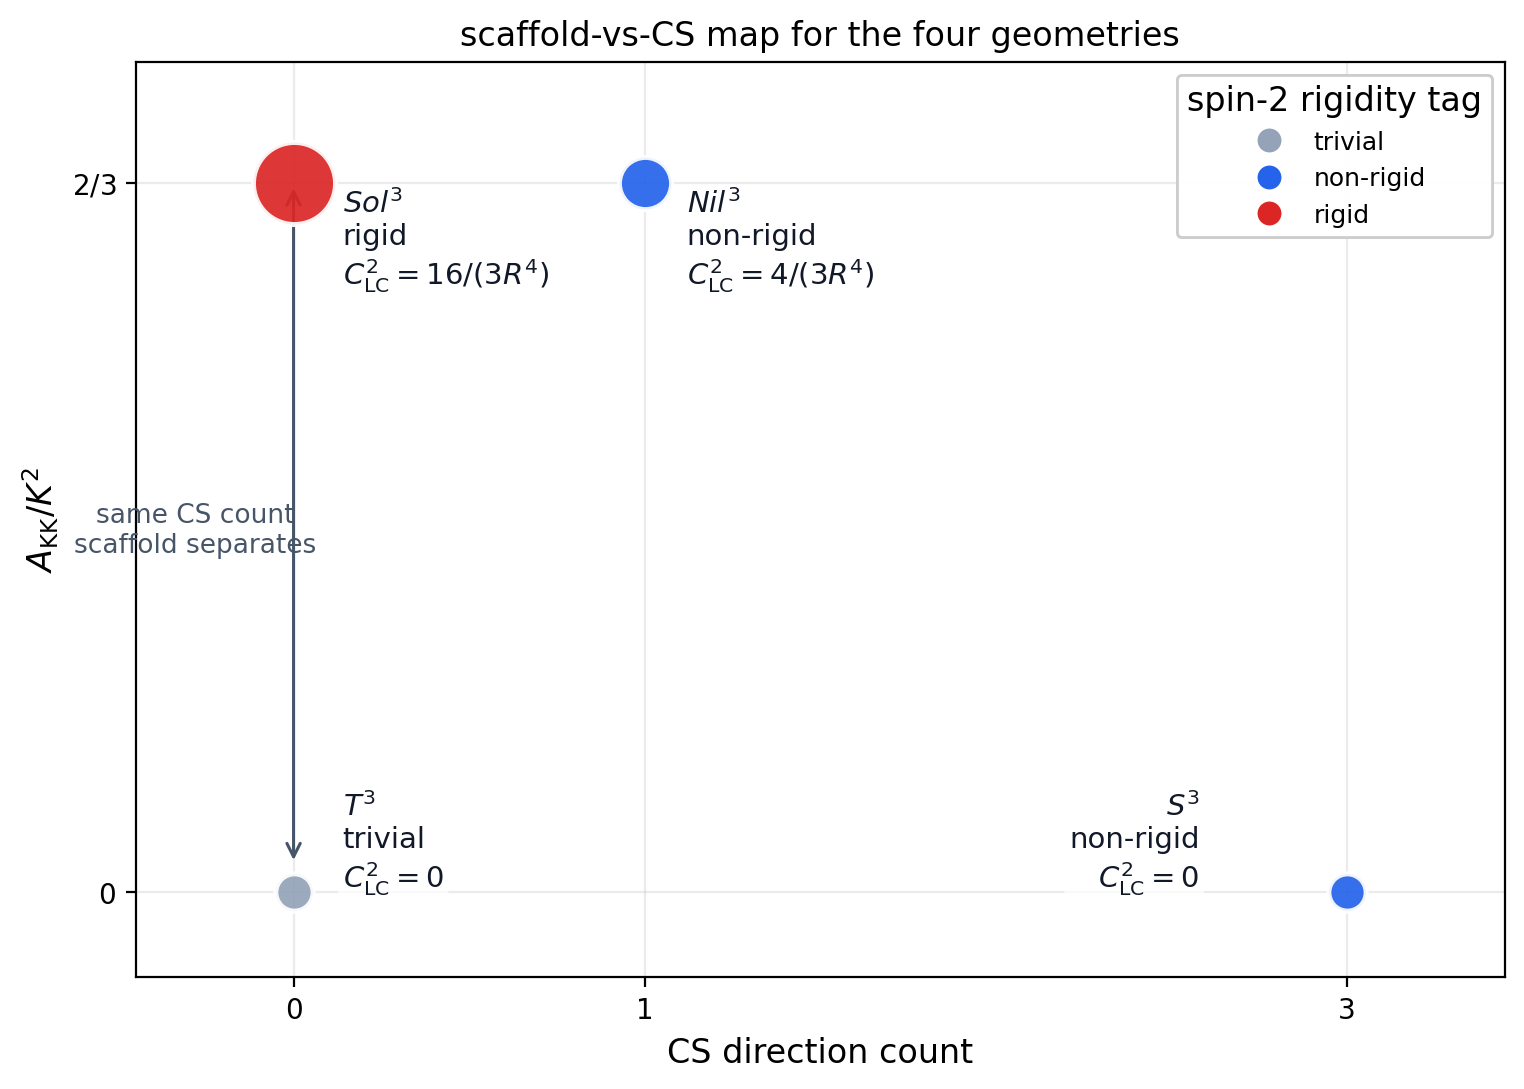
\includegraphics[width=0.85\linewidth]{figures/fig07_scaffold_vs_cs.png}
\caption{Scaffold-vs-CS scatter.  The horizontal axis is the CS direction
count, the vertical axis is $\AKK/K^2$, the marker size encodes
$C^2_\LC$, and the colour encodes the spin-2 rigidity tag.  $\Tthree$ and
$\Solthree$ share CS count $0$ but separate in the scaffold layer.}
\label{fig:scaffold}
\end{figure}

The spin-2 rigidity tag is not a strict numerical invariant but a
scaffold label summarising the zero pattern of the squash/shear Hessian.
``Rigid'' refers to the $\Solthree$ frame rigidity
\begin{equation}
  \frac{\partial^2 V}{\partial \varepsilon^2}
  = \frac{\partial^2 V}{\partial s^2}
  = \frac{\partial^2 V}{\partial \varepsilon\, \partial s} = 0,
\end{equation}
``trivial'' to the flat kinematic zero of $\Tthree$, and ``non-rigid'' to the
non-zero spin-2 Hessian of $\Nilthree$ / $\Sthree$.

This Hessian zero pattern is a non-trivial consequence of the fact that the
volume-preserving deformation
$f_1=(1+\varepsilon)^{2/3}(1+s),\ f_2=(1+\varepsilon)^{-2/3}/(1+s)$
of $\Solthree$ leaves the structure constants independent of $\varepsilon, s$
(Appendix~\ref{app:E:E1}); the script \texttt{proofs/sol3\_structure.py}
verifies that the three second derivatives vanish directly.

The KK anisotropy is defined as
\begin{equation}
  \AKK := \sum_{i=0}^{2}(m_i^2-\bar m^2)^2,
  \qquad
  \bar m^2 := \frac{1}{3}\sum_{i=0}^{2} m_i^2,
\end{equation}
normalised by $K^2 := \KMxw^2$; we record
$\AKK/K^2 = 0,\,2/3,\,0,\,2/3$ as the scaffold datum.

The role of this layer is not to add a new observable family but to explain
``why the activation pattern of the three families differs across the
geometries''.  Both $\Tthree$ and $\Solthree$ lack a local CS core, yet they
are separated in the bulk layer by the presence/absence of an EC slice
minimum and a rigid scaffold, and they are further distinguished in the
boundary layer by the global spectral branch dependent on the compact
quotient and spin structure.  On the Sol-A benchmark a trivial spectral
profile coincident with $\Tthree$ appears, whereas the Sol-P benchmark
raises a global spectral branch with $\etaAPS = 1$.  The geometric
distinction---that $\Tthree$ is flat and inert while $\Solthree$ carries a
non-vanishing Weyl curvature, an EC slice minimum, a biaxial KK splitting,
and frame rigidity---persists nonetheless.  This distinction does not
amount to introducing further observable families, but it is indispensable
for a complete characterisation of the geometries.

The second-layer dictionary thus closes through the three views:
geometry-wise, pairwise, and scaffold.  In the next section we combine these
with the bulk layer and compress the contents into selection rules instead of
an enumeration of individual computations.
   % Boundary / interface response
%==============================================================================
% Section 5: Selection rules
%==============================================================================
\section{Selection Rules}
\label{sec:rules}

This section compresses the results of \S\S\ref{sec:baseline}--\ref{sec:boundary}
into selection rules.  What matters is less the detail of individual
computations than a rule set surveying ``which response is allowed,
protected, or activated in which geometry''.  The selection rules are not a
restatement of the inventory; they translate the comparison of the four
geometries into reusable decision rules.

\subsection{Bulk Rules}
\label{sec:rules:bulk}

The principal rules of the bulk layer can be summarised as follows.  The
geometric origin of each rule is collected first in the following table.

\begin{table}[H]
\centering
\begin{tabular}{ll}
\toprule
Rule & Geometric source \\
\midrule
R1 & geometry-independence of the Maxwell action \\
R2 & presence/absence of off-diagonal structure constants \\
R3 & mass-splitting pattern of the KK vector sector \\
R4 & EC slice-minimum branch in the scalar potential \\
R5 & localisation well opened by the reduced 1D $\eta$-benchmark and its activation conditions \\
\bottomrule
\end{tabular}
\caption{Geometric source of each bulk rule.}
\label{tab:bulk_rules_source}
\end{table}

\paragraph{R1: Maxwell universality.}
The Maxwell baseline is common to the four geometries:
\begin{equation}
  \KMxw = -\frac{L^2}{2r_0^4}
\end{equation}
is the master coefficient for all four.  Geometry dependence is therefore
not in the kinetic baseline but on the side of the activated channels.

\textit{Justify.}  The principal part of Maxwell originates from the abelian
quadratic term $F_{ij}F^{ij}$, while the structure constants enter only the
lower-order mass / CS terms via the modified field strength.  Under the
common product-circle convention, the principal coefficient is therefore
fixed to $-L^2/(2r_0^4)$ for all four geometries (Appendix~\ref{app:E:E2b};
verification: \texttt{proofs/kk\_higgsing.py}).

\paragraph{R2: CS activation rule.}
The Chern--Simons channel is activated only when the correction to
$\tilde{F}_{ij}$ has its leg outside $\{i,j\}$.  $\Nilthree$ (one direction)
and $\Sthree$ (three directions) follow this rule; the self-referential
correction of $\Solthree$ cancels exactly.

\textit{Justify.}  Classifying the correction type into ``no structure
constant / off-diagonal / self-referential'' fixes the CS direction count
algebraically as $0/1/3/0$ (Appendix~\ref{app:E:E4}).  In $\Solthree$ the
legs of $A_1\to\tilde{F}_{01}$ and $A_2\to\tilde{F}_{02}$ lie inside the
field-strength index pair, so the CS coefficient remains zero for any
profile-local coefficients $c_{01}(z), c_{02}(z)$ (verification:
\texttt{proofs/cs\_cancellation.py}).  This is a statement about the
profile-local reduced KK ansatz, not the derivation of the full
derivative-dependent inhomogeneous field equation.

\paragraph{R3: Higgsing classification.}
The KK Higgsing pattern is classified into the four types
none / uniaxial / triaxial / biaxial; in this order each is realised exactly
once by $\Tthree, \Nilthree, \Sthree, \Solthree$, providing the most direct
compression of the bulk-sector mode dictionary.

\textit{Justify.}  Direct computation of the KK mass dictionaries gives
massive counts $0, 1, 3, 2$, exactly exhausting the four types
(Appendix~\ref{app:E:E5}).

\paragraph{R4: EC slice-minimum rule.}
A horizontal evaluation of the homogeneous EC + NY + Weyl potential of the
current DPPU library across the four geometries shows that an EC slice
minimum on the $\eta=V=0$ section exists in $\Nilthree$ and $\Solthree$ and
is absent in $\Tthree$ and round $\Sthree$.  Hence $\Nilthree$ carries the
spin-0 entry where CS and EC simultaneously rise, while $\Solthree$ carries
the CS-inert but EC-active rigid entry.

\textit{Justify.}  Paper~III (EC) \cite{paper3ec} shows analytically
\begin{equation}
  r_0 = \frac{4\kappa}{\sqrt{3}}\sqrt{|\alpha|},
  \qquad
  |\kappa^2 \theta_\NY| < 1 \Rightarrow \text{full homogeneous local minimum}.
\end{equation}
For $\Solthree$ the same $r_0$ and the same Hessian criterion hold, with the
slice potential and $H_{RR}$ four times those of $\Nilthree$.  $\Tthree$ has
no isolated radial branch on the flat zero slice, and round $\Sthree$ has
non-zero slope and no stationary point (Appendix~\ref{app:E:E5b};
verification: \texttt{paper04/ec\_slice\_minima.py}).

\paragraph{R5: reduced $\eta$-benchmark localisation rule.}
On the reduced 1D AX-torsion benchmark over a slice-wise homogeneous
background, the Gaussian radial dip produces a localisation well in all four
geometries.  Progress to a local parity-odd activated response, however,
requires CS-active structure.  Hence $\Nilthree$ is activated by CS+EC,
$\Sthree$ by CS+triplet/nonlinear opening, $\Tthree$ is kinematic / trivial,
and $\Solthree$ is EC-supported but CS-inert.

\textit{Justify.}  The current \texttt{dppu} library yields the exact
homogeneous datum
\begin{equation}
  M_{\mathrm{geo}} = \left.\frac{\partial^2 \Veff}{\partial \eta^2}\right|_{\eta=0}
  = c_{\mathrm{geo}}\,\rho,
\end{equation}
and the reduced 1D kinetic datum from the AX contortion gradient agrees:
$K_{\mathrm{geo}} = c_{\mathrm{geo}}\,\rho$, with
$c_{\Tthree} = c_{\Nilthree} = c_{\Solthree} = 96\pi^4 L/\kappa^2$ and
$c_{\Sthree} = 12\pi^2 L/\kappa^2$.  The variational evaluation for a
Gaussian $\rho$-dip then guarantees at least one bound state analytically
for all four geometries, and the representative benchmark scan confirms
LOCALIZED in all $4 \times 3 = 12$ examples
(Appendix~\ref{app:E:E6}; verification:
\texttt{paper04/eta\_defect\_coefficients.py},
\texttt{paper04/defect\_localization.py}).
The differences in response are determined not by localisation itself but by
whether CS activation (R2), the EC slice minimum (R4), or the
triplet/nonlinear opening is present in the subsequent stage: $\Nilthree$
has CS+EC, $\Sthree$ has CS+triplet, $\Solthree$ has EC alone, and $\Tthree$
has none.

The bulk rules above show that the four geometries can be compared in the
form ``universal baseline + geometry-dependent activation pattern''.  In
particular, $\Solthree$ does not introduce a CS-active family but, since it
carries an EC slice minimum, is not placed in the same minimal bulk class as
$\Tthree$.  $\Solthree$ remains as the CS-inert, EC-active, rigid geometry.

\subsection{Boundary Rules}
\label{sec:rules:boundary}

The principal rules of the boundary/cobordism layer are as follows.

\paragraph{B1: CZ inflow activation rule.}
The CZ inflow is activated only in CS-active geometries.  The torsion-CS
sector vanishes in $\Tthree$ and $\Solthree$ and a non-trivial inflow
remains only in $\Nilthree$ and $\Sthree$.

\textit{Justify.}  $\SCZ\propto\int\Ctor$ is non-zero only when the bulk CS is
active, in one-to-one correspondence with the CS direction count
$0/1/3/0$ of R2.

\paragraph{B2: local spectral-core rule.}
A strict local APS spectral core appears representatively in $\Nilthree$
with canonical value
\begin{equation}
  \etaAPS(\Nilthree) = +\frac{1}{2}.
\end{equation}
This entry belongs to the spinor spectral family and must not be conflated
with the torsion-CS family.

\textit{Justify.}  The Heisenberg mode decomposition shows $h=0$ for PPA and
that only the $n=0$ spin-up branch carries the asymmetry.  The value is
fixed by the Levi--Civita spinor CS integral $\int_Y\Csig = -1/2$ together
with the orientation convention $\etaAPS = -\int_Y\Csig$, giving
$\etaAPS = +1/2$ and $\eta(0) = 1$ (Appendix~\ref{app:E:E10};
verification: \texttt{paper04/eta\_aps\_nil3.py}).  As benchmarks, the PPA
$\Tthree$ and the round $\Sthree$ Levi--Civita Dirac have spectra exactly
symmetric under $\lambda\leftrightarrow -\lambda$, so $\etaAPS = 0$
(verification: \texttt{proofs/aps\_zero\_t3\_s3.py}).  On the compact
$\Solthree$ benchmark the local CS integral vanishes, but $\etaAPS$
branches as $1/0$ between Sol-P and Sol-A; $\Solthree$ is therefore treated
as a global spectral branch rather than a local core
(Appendix~\ref{app:E:E10b}; verification:
\texttt{proofs/eta\_aps\_sol3.py}).

\paragraph{B3: torsional-charge rule.}
The torsional-charge entry appears representatively in $\Sthree$ with
canonical value
\begin{equation}
  \Ntop = 6 r_0^2.
\end{equation}
This is the reason that pairs containing $\Sthree$ are torsional-charge-led
in the pairwise cobordism dictionary.

\textit{Justify.}  Starting from the structure constants
$C^i{}_{jk} = (4/r_0)\,\epsilon^i{}_{jk}$ of $\Sthree$, one obtains
$T^i = \tfrac{1}{2}C^i{}_{jk}\,e^j\wedge e^k$,
$\Ctor = (12/r_0)\,\mathrm{vol}_{\Sthree}$, and hence
$\int_{\Sthree}\Ctor = 24\pi^2 r_0^2$.  Dividing by the frame-bundle
normalisation $1/(4\pi^2)$ ($\pi_3(SO(3)) = \mathbb{Z}$, $T_R = 1$) gives
$\Ntop = 6 r_0^2$ (Appendix~\ref{app:E:E9}; verification:
\texttt{paper04/torsional\_charge.py}).

\paragraph{B4: spectral-source rule.}
Within the spectral family, one must distinguish not only the presence/absence
of the observable but also the source mechanism.  $\Nilthree$ has a local
spectral core supported by a non-zero Levi--Civita spinor CS integral, while
$\Solthree$ may have a global spectral branch sourced by kernel data
depending on the compact quotient and spin structure.

\textit{Justify.}  In $\Nilthree$, $\int_Y\Csig = -1/2$ directly fixes
$\etaAPS = +1/2$ (B2).  In $\Solthree$ on the compact mapping-torus
benchmark $M_A = T^2\rtimes_A \Sone$ the local CS integral remains
$\int_Y\Csig = 0$, while constant spinors in the $k=0$ sector descend only
under Sol-P, giving $h = 2/0$ and (with antilinear symmetry $\eta(0)=0$)
$\etaAPS(\text{Sol-P/Sol-A}) = 1/0$ (Appendix~\ref{app:E:E10b};
verification: \texttt{proofs/eta\_aps\_sol3.py}).  Hence $\Nilthree$ and
$\Solthree$ share the spectral family but not the same source.

\subsection{Pairwise Rules}
\label{sec:rules:pairwise}

The pairwise cobordism dictionary furnishes the following rules.

\begin{itemize}
  \item Pairs containing $\Sthree$ tend to be torsional-charge-led.
        $\Sthree$ carries the canonical frame-bundle-normalised
        torsional-charge core in the second layer (B3) and the bulk side
        possesses an isotropic activation structure (3-direction CS +
        triplet degeneracy, R2/R3).  However,
        $\Sthree\leftrightarrow\Solthree$ is torsional-charge-led on Sol-A
        and a torsional / global-spectral mixed pair on Sol-P.
  \item Pairs containing $\Nilthree$ tend to be spectrally led.  In
        $\Tthree\leftrightarrow\Nilthree$ the local APS core is the subject
        of comparison; in $\Nilthree\leftrightarrow\Solthree$ the
        ``local vs.\ global'' source distinction within the spectral family
        becomes the subject.  This is because $\Nilthree$ carries both an EC
        slice minimum (R4) and CS-active structure, and is the only Levi--Civita
        Dirac PPA case with a non-zero local CS core
        (Appendices~\ref{app:E:E10},~\ref{app:E:E10b}).  $\Solthree$ also
        carries an EC slice minimum but no local CS core, so its source
        mechanism is not identical to that of $\Nilthree$.
  \item $\Sthree\leftrightarrow\Nilthree$ is the representative mixed pair
        crossing the torsional-charge family ($\Ctor$) and the local
        spectral family ($\Csig$).  Since the two belong to different
        3-form sectors, they cannot be reduced to a single scalar
        observable (3-form distinction: Appendix~\ref{app:E:E8}).
  \item $\Tthree\leftrightarrow\Solthree$ is not a uniformly inert minimal
        pair but a benchmark pair sensitive to compact quotient / spin
        structure.  Sol-A coincides with the trivial spectral profile of
        $\Tthree$, while Sol-P raises a global spectral branch with
        $\etaAPS = 1$.  The scaffold differences ($C^2_\LC$, spin-2
        rigidity tag, $\AKK/K^2$) are preserved in both.
\end{itemize}

\subsection{Spectral Source and Geometric Distinctness}
\label{sec:rules:source}

A particularly important point about the selection rules is to avoid
conflating ``belonging to the same family'' with ``the value being
determined by the same source''.  Both $\Nilthree$ and $\Solthree$ may
appear in the spectral family, yet $\Nilthree$ is fixed by the local
Levi--Civita CS integral while $\Solthree$ is fixed by global kernel data
depending on compact quotient / spin structure.  The same spectral family
does not imply the same mechanism.

$\Tthree$ is flat and inert, while $\Solthree$ carries a non-vanishing Weyl
curvature, biaxial KK splitting, and frame rigidity.  Even where Sol-A makes
the boundary observable coincide with the $\Tthree$ trivial benchmark, the
background geometries do not coincide.  Conversely, on Sol-P a global
spectral branch is added and $\Solthree$ separates from $\Tthree$ already
at the second layer.  This distinction does not require introducing a
third or fourth observable family but reflects differences in the geometric
scaffold and global spectral sourcing that support the observables.  The
selection rules of this paper therefore deliberately separate ``compression
of observable classes'' from ``characterisation of background geometry''.

\subsection{Summary}
\label{sec:rules:summary}

By bringing the selection rules to the foreground, the inventory becomes
readable as a comparison structure linked to geometry-dependent rules.  The
next section retains this principal structure and discusses two readings of
the Euclidean circle.
   % Selection rules
%==============================================================================
% Section 6: Secondary readings of the Euclidean circle
%==============================================================================
\section{Secondary Readings of the Euclidean Circle}
\label{sec:circle}

This section organises two readings of the Euclidean circle $\Sone$.  These
provide a reduced description and a thermal description on top of the
already constructed Euclidean response dictionary.  Crucially, the readings
discussed here do not replace the main dictionary; they supply secondary
interpretations of the same Euclidean data.

\subsection{KK Reduction Reading}
\label{sec:circle:kk}

In the KK reading we distinguish the geometric response itself from the
reduced descriptor that describes it in lower-dimensional language.  The
effective coefficients and parity-odd channels appearing in the
lower-dimensional sector are images of the dictionary already constructed,
not the primary objects themselves.

We also fix the geometric setup used in the KK reduction normalisation
identity.  When extracting coefficients we treat the Euclidean circle as a
product/collar direction of length $\beta$ and apply the CZ identity
$\mathrm{NY} = \dd\Ctor$ together with Stokes' theorem on the relative
cobordism
\begin{equation}
  X^4 = M^3 \times I_\beta, \qquad I_\beta = [0, \beta].
\end{equation}
The 3D effective coefficient is defined as a functional on a single physical
boundary slice $Y = M^3$ that absorbs the volume factor along $I_\beta$, so
that here $\int_{\partial X^4}\Ctor$ refers to this single-copy boundary
contribution.  The coefficient $k_{3D}^{\mathrm{tor\text{-}CS}}$ is therefore
the 3D boundary coefficient obtained under inflow/collar normalisation, not
a two-endpoint difference along a closed thermal trace.  Where the
cancellation of the non-zero KK tower is invoked, we assume a real bosonic
KK decomposition on an untwisted product circle.

For this reduced-side reading the following three consistency statements are
useful:
\begin{equation}
  k_{3D}^{\mathrm{tor\text{-}CS}} = \frac{1}{2}\,k_{4D}^{\NY},
  \qquad
  Q_{\mathrm{best}} := \frac{\eta(0)}{\Delta k_{\mathrm{matter}}} = 1,
  \qquad
  k_q \in \mathbb{Z}.
\end{equation}
The first two give normalisation-free statements about the
torsional / matter-coupled parity-odd descriptors, and the last gives the
integrality condition for the reduced Chern--Simons level.

The first identity $k_{3D}^{\mathrm{tor\text{-}CS}} = (1/2)k_{4D}^{\NY}$ is
obtained algebraically as the 3D torsion-CS level after KK reduction along
$\Sone$ of the 4D Nieh--Yan action
$S_\NY = (k_{4D}^{\NY}/8\pi^2)\int \dd\Ctor$
(KK reduction normalisation identity; Appendix~\ref{app:E:E11};
verification: \texttt{proofs/kk\_normalization.py}).  Here, on an untwisted
product circle, the Fourier modes $n$ and $-n$ form complex-conjugate pairs
and the even weights are determined by $n^2$ alone, so that the parity-odd
residue takes the form $n\,w(n^2)$.  The non-zero tower therefore cancels
pairwise and leaves no further parity-odd shift.  The second identity
$Q_{\mathrm{best}} = 1$ follows from the comparison between the spinor-CS
and the APS spectral entry: in $\Nilthree$ one has $\eta(0) = 1$ and
$\Delta k_{\mathrm{matter}} = 1$ (matter-minimal inflow audit;
Appendix~\ref{app:E:E12}).  The third statement $k_q\in\mathbb{Z}$ is the
formal quantisation condition required by large gauge transformations
on the frame bundle, $\pi_3(SO(3)) = \mathbb{Z}$ (formal quantisation on the
frame bundle; Appendix~\ref{app:E:E13}).  These are not new observable
families of the second layer but consistency statements that arise when the
Euclidean response is read in lower-dimensional language.

On the bulk side, the universal Maxwell coefficient
\begin{equation}
  \KMxw = -\frac{L^2}{2r_0^4}
\end{equation}
is reread as a topology-independent kinetic baseline, while the activated
Chern--Simons directions, the uniaxial Higgsing of $\Nilthree$, and the
triplet degeneracy of $\Sthree$ are interpreted as topology-dependent
channels of the reduced vector sector.  The reduced language is therefore a
re-reading of the bulk inventory in lower-dimensional form, not something
prior to the bulk inventory.

On the boundary side, the torsional inflow action, the APS spectral entry,
and the frame-bundle-normalised torsional charge can likewise be mapped to
parity-odd descriptors in lower-dimensional language.  However, $\SCZ$ is
written in terms of $\Ctor$ while $\etaAPS$ belongs to Levi--Civita
spectral data, so the observable-family distinction is preserved even after
projecting onto reduced language.  In particular,
$\etaAPS(\Nilthree) = 1/2$ and $\Ntop(\Sthree) = 6 r_0^2$ both admit
reduced parity-odd descriptors but are not the same quantity.  We do not
claim a complete identification between the reduced-side statements and the
native geometric quantities.

In this sense the KK language does not replace the response dictionary; it
provides a reduced reading of it.  The coefficient correspondences and the
normalisation chain are collected in Appendix~\ref{app:D}.

\subsection{Matsubara-Style Thermal Reading}
\label{sec:circle:matsubara}

In order to overlay a thermal-descriptor reading on the same Euclidean
circle, we adopt
\begin{equation}
  \beta = L
\end{equation}
and describe a Matsubara-style thermal reading as the thermal interpretation.
Here $L$ is the same length of the Euclidean circle that already appears in
the geometric formulation; the thermal reading does not introduce a new
circle but assigns thermal meaning to the existing Euclidean data.

Under this interpretation, Maxwell universality, the CS direction-count law,
the uniaxial Higgsing of $\Nilthree$, and the triplet degeneracy of
$\Sthree$ remain Euclidean structural entries; only the thermal-descriptor
language is added to them.  Moreover, the Matsubara reading does not break
the original product structure $M^3\times \Sone$, so it does not by itself
generate a new parity-odd source.  In this sense, what we obtain is a
$P=0$-protected thermal sector, not a full Lorentzian continuation.

The KK reading and the Matsubara-style thermal reading coexist as two
secondary readings of the same Euclidean circle.  Coexistence on the same
circle, however, does not imply theoretical identity: the former is a
lower-dimensional descriptor language and the latter is a thermal
descriptor language, and the reduced gauge coefficient, boundary inflow
action, phase labels, etc.\ merely admit both readings.

The thermal reading of this section is deliberately confined to the
Euclidean scope.  We do not claim a derivation of full finite-temperature
field theory, a strict construction of the partition function, a detailed
analysis of the Matsubara sum, or real-time transport.  The KK--Matsubara
coexistence table is collected in Appendix~\ref{app:C}, and the descriptor
separation and normalisation chain in Appendix~\ref{app:D}.
   % Secondary readings of the Euclidean circle
%==============================================================================
% Section 7: Discussion and Outlook
%==============================================================================
\section{Discussion and Outlook}
\label{sec:discussion}

This section organises the implications of the results and the directions
for future work.

\subsection{What This Paper Has Fixed}
\label{sec:discussion:fixed}

This paper fixes a fairly strong dictionary---rather than the bare
minimum---for placing the four Thurston geometries within a single
comparison framework.  In the first layer the 36-entry bulk inventory closes,
making explicit that geometry-dependent activation rules ride on top of
Maxwell universality.  In the second layer the three observable families
spectral / torsional-charge / inflow are clearly separated, and the pairwise
cobordism dictionary organises all six pairs into a comparable form.

This organisation positions $\Nilthree$ as the geometry that carries a
strict local APS spectral core, $\Sthree$ as the geometry that carries a
frame-bundle-normalised torsional-charge core, $\Tthree$ as the trivial
spectral benchmark, and $\Solthree$ as the geometry that may carry a global
spectral branch depending on the compact quotient and spin structure.  An
important point is that within the spectral family one must still
distinguish sources: the value in $\Nilthree$ is fixed by the local
Levi--Civita spinor CS, while the spectral entry in $\Solthree$ is raised
by global kernel / spin data.  The scaffold layer is needed to describe
this difference of source together with the distinctness of the background
geometries simultaneously.

By aligning a KK reading and a Matsubara-style thermal reading on the same
Euclidean circle we have also made explicit that, with the main dictionary
preserved, a reduced description and a thermal description can be added.
This shows that the principal result of this paper is the Euclidean
response dictionary itself, while the two readings are secondary
interpretations of it.

\subsection{Future Directions}
\label{sec:discussion:future}

Direct extensions split into at least the following three lines.

\begin{enumerate}
  \item \textbf{Lorentzian extension.}  Lifting the Euclidean response
        dictionary fixed here to a Lorentzian setting may make it possible
        to decide which protected / activated structure survives as a
        real-time observable.  In particular, which of parity-odd transport,
        interface response, and thermal interpretation will withstand
        analytic continuation is the next-stage question to be made
        explicit.

  \item \textbf{Application to phenomenology.}  The dictionary is not
        confined to abstract geometry classification but can serve as a
        platform that organises which response channels are expected for
        phenomenological labels such as metastable, rolling, or no-support
        branches.  Using bulk activation and boundary observables together
        leaves room for organising geometry dependence that is invisible
        from a single effective coefficient.

  \item \textbf{Generalisation of $\Solthree$ compact-quotient / spin-structure
        dependence.}  This paper makes the boundary spectral entry of
        $\Solthree$ strict on a compact mapping-torus benchmark, but how
        the kernel structure changes for general hyperbolic monodromies and
        quotient families is left for future work.  Making explicit how the
        local/global dichotomy fixed here generalises across the Sol family
        is the natural next step for handling borderline spectral entries.
\end{enumerate}
   % Discussion and Outlook
%==============================================================================
% Section 8: Conclusion
%==============================================================================
\section{Conclusion}
\label{sec:conclusion}

In this paper we have constructed a Euclidean geometric response dictionary
and the corresponding selection rules for the four Thurston geometries
$\Tthree$, $\Nilthree$, $\Sthree$, and $\Solthree$.  The principal result is
the organisation of the response into a two-layer structure that closes the
bulk inventory and the boundary/cobordism inventory across the four
geometries.

In the first layer we provided a 36-entry bulk inventory and its selection
rules.  Here the Maxwell coefficient
\begin{equation}
  \KMxw = -\frac{L^2}{2r_0^4}
\end{equation}
is common to the four geometries, while the activation conditions for CS,
the Higgsing pattern, the EC slice-minimum structure, and the reduced
$\eta$-mode defect-localisation benchmark branch in a geometry-dependent
manner.  $\Nilthree$ is organised as a CS+EC activated geometry, $\Sthree$
as the most richly CS- and Higgsing-activated geometry, $\Tthree$ as an
inert benchmark, and $\Solthree$ as a CS-inert / EC-active geometry with a
rigid scaffold.

In the second layer we fixed the three observable families spectral,
torsional-charge, and inflow, together with the pairwise cobordism
dictionary.  In particular, the strict local APS core of $\Nilthree$, the
frame-bundle-normalised torsional-charge core of $\Sthree$, the trivial
spectral benchmark of $\Tthree$, and the spin-sensitive global spectral
branch on the compact $\Solthree$ benchmark constitute the centre of the
comparison dictionary.  This makes explicit the separation of local and
global sources within the spectral family.  The geometric scaffold layer
distinguishes this difference of source from the distinctness of the
background geometry.

We have further presented two readings of the Euclidean circle, the KK
reduction reading and the Matsubara-style thermal reading.  These provide a
reduced description and a thermal description respectively, but are not
identified theoretically.  They coexist as secondary interpretations of the
already constructed Euclidean response dictionary.

In conclusion, the present paper offers a Euclidean geometric response
dictionary that gives the allowed, protected, and activated responses of the
four geometries as a coherent rule set.  The principal contribution is the
explicit display of how the layers of bulk, boundary, cobordism, and circle
readings are organised once the four Thurston geometries are placed within
the same comparison framework.
   % Conclusion

%------------------------------------------------------------------------------
% Acknowledgments
%------------------------------------------------------------------------------
\section*{Acknowledgments}

The author acknowledges the use of the following AI tools during manuscript
preparation: Claude Opus~4.7 (Anthropic; accessed 2026-04),
Gemini~3.1 Pro (Google; accessed 2026-04), Grok 4.3 (xAI; accessed 2026-04),
and GPT-5.5 Thinking via ChatGPT (OpenAI; accessed 2026-04).
These tools were used for language editing (including Japanese--English
translation), outlining and improving exposition, drafting and reviewing
auxiliary code (scripts and pseudocode) that was subsequently tested and
validated by the author, and proposing candidate consistency checks and
alternative derivations to be independently verified by the author.

The AI tools did not determine the scientific claims of this work and were not
used to generate or modify research data or evidentiary figures.  The author
takes full responsibility for the content and for any remaining errors.

This work was developed within the informal collaborative project
\textbf{DPPU} (\textbf{D}onut-like topology, \textbf{P}lanck-scale
compactness, \textbf{P}recession dynamics, \textbf{U}niverse).

%------------------------------------------------------------------------------
% Availability and Contact
%------------------------------------------------------------------------------
\section*{Availability and Contact}

\paragraph{Code and Data Availability}
The code and supplemental data associated with this work are available at:

\begin{itemize}
  \item Zenodo: \texttt{10.5281/zenodo.19775695}
  \item GitHub: \texttt{https://github.com/Muacca/DPPUv7-paper04}
\end{itemize}

They are released under the MIT License.

\paragraph{Citation}
If you use these materials, please cite the associated manuscript and Zenodo record:

\begin{quote}
\small
Muacca, ``Euclidean Geometric Response Dictionary and Selection Rules for Four
Thurston Geometries.''
\end{quote}

\paragraph{Contact}
For questions, bug reports, or collaboration inquiries:

\begin{itemize}
  \item Email: \texttt{muacca@dmwp.jp}
  \item GitHub Issues: \texttt{https://github.com/Muacca/DPPUv7-paper04/issues}
\end{itemize}

%------------------------------------------------------------------------------
% Appendices
%------------------------------------------------------------------------------
\appendix
%==============================================================================
% Appendix A: Notation and Conventions
%==============================================================================
\section{Notation and Conventions}
\label{app:A}

This appendix collects the notation conventions used in the body, the
shorthand for the four geometries, the terminology of the two-layer
structure, and the distinction between three 3-forms that are easily
conflated.  Since the formulas in the body are written in compact form, the
premises of the comparison are made explicit here.

\subsection{Geometries and Common Setup}
\label{app:A:geom}

\begin{itemize}
  \item $\Tthree$: flat three-torus.
  \item $\Nilthree$: Heisenberg-type nil geometry.
  \item $\Sthree$: round three-sphere.
  \item $\Solthree$: solv geometry.
\end{itemize}

In this paper ``the four geometries'' always refer to these four.  All
comparisons are carried out on the Euclidean product structure
\begin{equation}
  M^3 \times \Sone,
\end{equation}
with $L$ denoting the length of $\Sone$.  $r_0$ is the reference length
characterising the homogeneous background, and $R$ is the geometric scale
appearing in the structure constants of the three-dimensional spatial part.

\subsection{Two-Layer Structure and Response Vocabulary}
\label{app:A:layer}

\begin{itemize}
  \item \textbf{first layer}: response that can be defined on the bulk side
        without introducing a boundary.
  \item \textbf{second layer}: response defined in the
        boundary / interface / cobordism setting.
  \item \textbf{secondary reading}: an interpretive layer that re-reads, in
        another language, the already-fixed Euclidean response dictionary.
\end{itemize}

In the body we further use the following terms.

\begin{itemize}
  \item \textbf{allowed}: the channel is geometrically meaningful.
  \item \textbf{protected}: the channel is not automatically opened even
        under non-trivial perturbations.
  \item \textbf{activated}: a non-trivial response is raised by the
        structure of the geometry.
  \item \textbf{minimal}: there is no active family and the geometry sits
        on the benchmark side.
\end{itemize}

\subsection{Principal Symbols and Representative Values}
\label{app:A:symbols}

\begin{itemize}
  \item $\KMxw$: Maxwell baseline coefficient.
  \item $\SCZ$: Callias--Zanelli inflow action.
  \item $\etaAPS$: APS spectral invariant.
  \item $\Ntop$: frame-bundle-normalised torsional-charge entry.
  \item $C^2_\LC$: Levi--Civita Weyl scalar.
  \item spin-2 rigidity tag: scaffold-layer label
        (\texttt{trivial / non-rigid / rigid}).
  \item $\AKK$: KK anisotropy marker.
  \item AX torsion ansatz: $T_{ijk} = (2\eta/\rho)\,\epsilon_{ijk}$
        (DPPU AX-mode convention from paper~III (EC) \S3; the coefficient
        $2/\rho$ is fixed by this convention).
\end{itemize}

Representative benchmark values are listed below.  Derivation sketches and
verification scripts are referenced in Appendix~\ref{app:E}.

\begin{table}[H]
\centering
\resizebox{\linewidth}{!}{%
\begin{tabular}{lccl}
\toprule
Quantity & Value & Role & Derivation \\
\midrule
$\KMxw$ & $-L^2/(2 r_0^4)$ & universal bulk baseline & \S\ref{app:E:E2}, \S\ref{app:E:E5} \\
$\etaAPS(\Nilthree)$ & $+1/2$ & strict spectral core & \S\ref{app:E:E10} \\
$\Ntop(\Sthree)$ & $6 r_0^2$ & frame-bundle-norm.\ torsional-charge core & \S\ref{app:E:E9} \\
EC slice branch & present for $\Nilthree, \Solthree$ & spin-0 bulk branch & \S\ref{app:E:E5b} \\
$m^2(A_1) = m^2(A_2)$ in $\Solthree$ & $-L^2/(2 r_0^4)$ & biaxial KK splitting & \S\ref{app:E:E2}, \S\ref{app:E:E5} \\
$C^2_\LC(\Nilthree)$ & $4/(3 R^4)$ & scaffold datum & \S\ref{app:E:E7} \\
$C^2_\LC(\Solthree)$ & $16/(3 R^4)$ & scaffold datum & \S\ref{app:E:E7} \\
$k_{3D}^{\mathrm{tor\text{-}CS}}/k_{4D}^{\NY}$ & $1/2$ & NY--CS normalisation identity & \S\ref{app:E:E11} \\
$Q_{\mathrm{best}} = \eta(0)/\Delta k_{\mathrm{matter}}$ & $1$ & normalisation-free invariant & \S\ref{app:E:E12} \\
$k_q$ (formal) & $\in\mathbb{Z}$ & reduced CS level integrality & \S\ref{app:E:E13} \\
\bottomrule
\end{tabular}%
}
\caption{Representative benchmark values.}
\label{tab:appA_values}
\end{table}

\subsection{The Three 3-Forms and Their Connection}
\label{app:A:3forms}

We carefully separate the following 3-forms.

\begin{itemize}
  \item $\Ctor$: torsion-CS form.
  \item $\Csig$: spinor CS form.
  \item $\Cadj$: adjoint CS form.
\end{itemize}

The CZ inflow corresponds to $\Ctor$, and the APS spectral entry to $\Csig$.
In the body these must not be conflated.  Conceptually
\begin{equation}
  \mathrm{NY} = \dd\Ctor,
\end{equation}
and $\Cadj$ appears at intermediate stages of the APS argument.

\subsection{Geometric Scaffold Quantities}
\label{app:A:scaffold}

The following quantities, although not observable families themselves, are
used to record the distinctness of the background geometries.

\begin{itemize}
  \item $C^2_\LC$: magnitude of the Levi--Civita Weyl curvature.
  \item spin-2 rigidity tag: scaffold label summarising the zero pattern of
        the squash / shear Hessian.
  \item $\AKK / K^2$: magnitude of the KK anisotropy, with
        \begin{equation}
          \AKK := \sum_{i=0}^{2}(m_i^2 - \bar m^2)^2,
          \qquad
          \bar m^2 := \frac{1}{3}\sum_{i=0}^{2} m_i^2,
          \qquad
          K^2 := \KMxw^2.
        \end{equation}
\end{itemize}

This scaffold layer does not define an additional observable family, but it
is indispensable for distinguishing geometries such as $\Tthree$ and
$\Solthree$ that share the absence of a local CS core.  In particular,
$\Solthree$ is CS-inert yet carries an EC slice minimum and frame rigidity.

The benchmark values $\AKK / K^2$ can be computed directly from the mass
dictionaries:

\begin{itemize}
  \item $\Tthree$: $m_i^2 = 0$, so $\AKK / K^2 = 0$.
  \item $\Nilthree$ (uniaxial $m_2^2 = \KMxw$): $\bar m^2 = K/3$,
        $\AKK = 2(K/3)^2 + (2K/3)^2 = (2/3)K^2$.
  \item $\Sthree$ (triplet $m_i^2 = -2L^2/r_0^4$): all $i$ equal, so
        $\AKK / K^2 = 0$.
  \item $\Solthree$ (biaxial $m_1^2 = m_2^2 = \KMxw$): $\bar m^2 = 2K/3$,
        $\AKK = (2K/3)^2 + 2(K/3)^2 = (2/3)K^2$.
\end{itemize}

This symbolic confirmation is performed in
\texttt{proofs/kk\_higgsing.py}.
  % Notation and Conventions
%==============================================================================
% Appendix B: Full response inventories
%==============================================================================
\section{Full Response Inventories}
\label{app:B}

This appendix collects the full response inventories that appear in
summary form in the body.  Where the body compresses the tables for
readability, here the tables are gathered together for ease of comparison.

\subsection{Bulk Inventory}
\label{app:B:bulk}

\begin{table}[H]
\centering
\resizebox{\linewidth}{!}{%
\begin{tabular}{lcccc}
\toprule
Entry & $\Tthree$ & $\Nilthree$ & $\Sthree$ & $\Solthree$ \\
\midrule
Maxwell coefficient & $-L^2/(2 r_0^4)$ & $-L^2/(2 r_0^4)$ & $-L^2/(2 r_0^4)$ & $-L^2/(2 r_0^4)$ \\
CS direction count & 0 & 1 & 3 & 0 \\
KK Higgsing & none & uniaxial & triaxial & biaxial \\
EC slice minimum & absent & present & absent & present \\
spin-2 rigidity & non-rigid & non-rigid & non-rigid & rigid \\
$P$-linear transport & protected & activated & activated & protected \\
nonlinear opening & absent & absent & activated & absent \\
defect-localisation response ($\eta$ benchmark) & trivial & activated & activated & EC-supported / CS-inert \\
inhomogeneous bulk response & trivial & activated & activated & CS-inert / EC-active \\
\bottomrule
\end{tabular}%
}
\caption{Full bulk inventory.}
\label{tab:appB_bulk}
\end{table}

\begin{figure}[H]
\centering
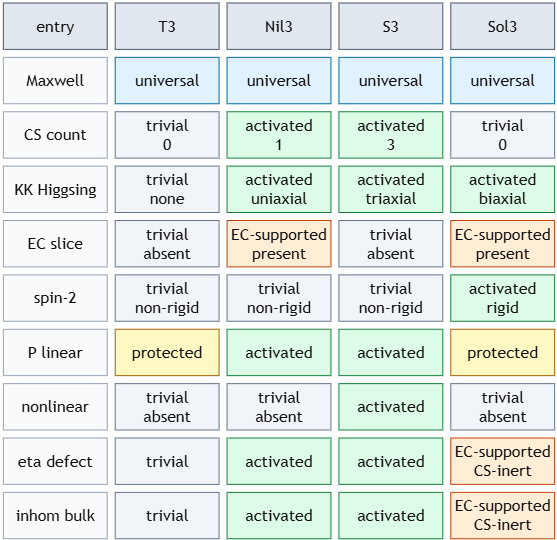
\includegraphics[width=0.95\linewidth]{figures/fig08_bulk_inventory_block.png}
\caption{36-entry bulk inventory block diagram.  The 9 entries $\times$ 4
geometries of \S\ref{app:B:bulk} are colour-coded as
\texttt{universal / activated / protected / trivial / EC-supported}.  In
particular, $\Solthree$ shares CS count $0$ with $\Tthree$, but in the EC
slice and inhomogeneous response rows it branches to the EC-supported side.}
\label{fig:bulk_block}
\end{figure}

The bulk inventory takes the form ``universal baseline + geometry-dependent
activation''.  $\Nilthree$ and $\Sthree$ progress as far as a local
parity-odd response on the activated side; $\Tthree$ is the minimal / inert
benchmark.  $\Solthree$ is CS-inert in the direction count but carries an EC
slice minimum and a rigid scaffold, so it is not placed in the same minimal
class as $\Tthree$.  The row ``defect-localisation response ($\eta$
benchmark)'' records not the existence of a bound state in the common
reduced 1D $\eta$-benchmark but how the localisation links to the additional
structure.

\subsection{Boundary Inventory}
\label{app:B:boundary}

\begin{table}[H]
\centering\small
\begingroup
\renewcommand{\arraystretch}{2.0}
\begin{tabularx}{\linewidth}{YXXXX}
\toprule
Entry & $\Tthree$ & $\Nilthree$ & $\Sthree$ & $\Solthree$ \\
\midrule
CS interface jump & absent & present & present & absent \\
APS spectral entry & $0$ & strict $+1/2$\newline (local) & $0$ & $0/1$\newline (Sol-A / Sol-P) \\
frame-bundle-norm. torsional charge $\Ntop$ & 0 & 0 & $6 r_0^2$ & 0 \\
CZ inflow & absent & activated & activated & absent \\
edge / interface response & minimal & activated & activated & spin-sensitive \\
boundary tag & trivial\newline benchmark & APS local\newline core & torsional-\newline charge active & global spectral\newline branch \\
\bottomrule
\end{tabularx}
\endgroup
\caption{Full boundary inventory.}
\label{tab:appB_boundary}
\end{table}

The strict observable of $\Nilthree$ belongs to the local spectral family,
that of $\Sthree$ to the torsional-charge family.  Furthermore, on the
compact mapping-torus benchmark, $\Solthree$ may carry a global spectral
branch.  This distinction is the key to understanding the mixed pairs and
source differences in the pairwise dictionary.

\subsection{Pairwise Cobordism Dictionary}
\label{app:B:pairwise}

\begin{table}[H]
\centering\small
\begingroup
\renewcommand{\arraystretch}{1.5}
\begin{tabularx}{\linewidth}{lXXX}
\toprule
Pair & Class & Dominant observable & Not-comparable note \\
\midrule
$\Sthree \leftrightarrow \Tthree$ & torsional / trivial & frame-bundle-norm.\ torsional charge & none \\
$\Sthree \leftrightarrow \Nilthree$ & torsional / local spectral & mixed & torsional-charge and local spectral are not the same quantity \\
$\Sthree \leftrightarrow \Solthree$ & torsional / global spectral & spin-sensitive & torsional-led for Sol-A; mixed for Sol-P \\
$\Tthree \leftrightarrow \Nilthree$ & trivial / local spectral & spectral & none \\
$\Tthree \leftrightarrow \Solthree$ & trivial / global spectral & spin-sensitive & Sol-A: trivial;\newline Sol-P: global spectral \\
$\Nilthree \leftrightarrow \Solthree$ & local / global spectral & spectral & source distinction within the spectral family \\
\bottomrule
\end{tabularx}
\endgroup
\caption{Full pairwise cobordism dictionary.}
\label{tab:appB_pairwise}
\end{table}

In the pairwise table the dominant observable supplies the subject of
comparison, and the ``not-comparable note'' makes explicit either that
direct subtraction is meaningless because the observable families differ,
or that the source differs even within the same spectral family.

\subsection{Strict Normalisation Cores}
\label{app:B:cores}

Together with the boundary observable families, the principal results of
this paper are supported by three strict normalisation cores.  These appear
in the reduced-side consistency statements of \S\ref{sec:circle:kk} but do
not define new second-layer observable families; they are native
quantities that guarantee the internal consistency of the Euclidean
response dictionary.

\begin{table}[H]
\centering\small
\begingroup
\renewcommand{\arraystretch}{1.5}
\begin{tabularx}{\linewidth}{clXYp{3.5cm}}
\toprule
\# & Core statement & Descriptor & Status & Verification \\
\midrule
C-1 & $k_{3D}^{\mathrm{tor\text{-}CS}} = \tfrac{1}{2}\,k_{4D}^{\NY}$ & $\Ctor$ inflow normalisation & strict (CZ + Stokes) & \S\ref{app:E:E11} \\
C-2 & $Q_{\mathrm{best}} = 1$ & doubly normalisation-free quotient & strict (matter assumption minimal) & \S\ref{app:E:E12} \\
C-3 & $k_q\in\mathbb{Z}$ & reduced CS level integrality & formal (single-valuedness) & \S\ref{app:E:E13} \\
\bottomrule
\end{tabularx}
\endgroup
\caption{Three strict normalisation cores.}
\label{tab:appB_cores}
\end{table}

\subsubsection{KK Reduction Normalisation Identity (C-1)}
\label{app:B:C1}

For the 4D Nieh--Yan action
$S_\NY^{(4D)} = (k_{4D}^{\NY}/8\pi^2)\int_{X^4}\mathrm{NY}$, applying the CZ
identity $\mathrm{NY} = \dd\Ctor$ together with Stokes' theorem on
$X^4 = M^3\times[0,\beta]$ gives, on the 3D boundary,
\begin{equation}
  S_{\mathrm{eff}}^{(3D)} \supset \frac{k_{4D}^{\NY}}{2}\cdot \Ntop.
\end{equation}
Hence the coefficient on the normalised basis
\begin{equation}
  \Ntop := \frac{1}{4\pi^2}\int_{M_3}\Ctor
\end{equation}
is fixed as the 3D torsion-CS coefficient,
\begin{equation}
  k_{3D}^{\mathrm{tor\text{-}CS}} = \frac{1}{2}\,k_{4D}^{\NY}.
\end{equation}
Here $\Ntop$ stands for the basis of the frame-bundle-normalised torsional
charge; since this paper imposes no extra quantisation condition on $r_0$,
no general integrality is claimed.  The factor $1/2$ originates from
$4\pi^2/8\pi^2$ and is independent of $r_0$.  Furthermore, on the untwisted
product circle the parity-odd residue from a real bosonic KK decomposition
takes the form $n\,w(n^2)$, so the contribution of the KK tower
($n\neq 0$) cancels strictly in pairs.  Detailed derivation and SymPy
verification are in Appendix~\ref{app:E:E11} and
\texttt{proofs/kk\_normalization.py}.

\subsubsection{Matter-Minimal Inflow Audit (C-2)}
\label{app:B:C2}

The quotient $Q_{\mathrm{best}} = \eta(0)/\Delta k_{\mathrm{matter}}$ is
formed from the numerator $\eta(0)^{(3D)} = 1$ (\S\ref{app:E:E10}) and the
denominator $\Delta k_{\mathrm{matter}} = h_{\mathrm{rep}}/2 = 1$
(Redlich parity shift \cite{Redlich1984}, $h_{\mathrm{rep}} = 2$).  Both are
\emph{doubly normalisation-free}:

\begin{itemize}
  \item the numerator is a spectral invariant that does not pass through
        the 4D APS bridge;
  \item the denominator depends only on $h_{\mathrm{rep}}$ and does not pass
        through the KK normalisation.
\end{itemize}

Hence $Q_{\mathrm{best}} = 1$ is a strict invariant independent of
normalisation conventions.  Details are in Appendix~\ref{app:E:E12}.

\begin{remark}
The Redlich parity shift is used here only as the standard
three-dimensional normalisation unit for the parity-odd level shift.
No dynamical fermion field is introduced in the geometric sector,
and the comparison is kept at the level of a translation-layer
normalisation audit.
\end{remark}

\subsubsection{Formal Quantisation on the Frame Bundle (C-3)}
\label{app:B:C3}

For the parity-odd effective action
$S_{\mathrm{odd}}^{(3D)} = k_q\cdot W[A/\omega]$ on the 3D boundary, the
single-valuedness $e^{i\Delta S_{\mathrm{odd}}} = 1$ requires, for the unit
winding shift under a large rotation on the frame bundle
($\pi_3(SO(3)) = \mathbb{Z}$),
\begin{equation}
  e^{2\pi i k_q} = 1 \iff k_q \in \mathbb{Z}.
\end{equation}
This gives a formal quantisation condition for the boundary Chern--Simons
level associated with the frame-bundle response. In the present work, this
condition is used as a boundary-level consistency criterion. Its complete
identification with the four-dimensional Nieh--Yan coupling
$\theta_{\rm NY}$ requires an additional normalization bridge between the
four-dimensional Nieh--Yan transgression and the three-dimensional
frame-bundle Chern--Simons functional. That bridge is not fixed here.
Accordingly, the statement $k_q\in\mathbb{Z}$ should be read as a formal
boundary quantisation condition, rather than as a first-principles derivation
of the $\theta_{\rm NY}$ normalization. Details are in Appendix~\ref{app:E:E13}.

\subsubsection{Cross-Audit Summary}
\label{app:B:cross}

C-1, C-2, and C-3 are cross-audited along three independent routes.  Here
``independent'' is restricted to the meaning ``no core uses the value of
another as input''.  Normalisation conventions such as $1/(4\pi^2)$,
$1/(8\pi^2)$, and $T_R = 1$ may be shared across cores, but this is a
common convention layer rather than circulation.  The inputs to each core
are listed below.

\begin{table}[H]
\centering\small
\begingroup
\renewcommand{\arraystretch}{1.5}
\begin{tabularx}{\linewidth}{@{}lY@{\hspace{1.2em}}Yc@{}}
\toprule
Core & Input from & \shortstack{Physical\\quantities} & \shortstack{Depends on\\other core?} \\
\midrule
C-1: $k_{3D}^{\mathrm{tor\text{-}CS}} = k_{4D}^{\NY}/2$ & 4D NY action + CZ + Stokes & $\Ctor$, $\Ntop$ basis & NO \\
C-2: $Q_{\mathrm{best}} = 1$ & spinor APS ($\eta(0) = 1$) + Redlich shift ($h_{\mathrm{rep}} = 2$) & $\Csig$ & NO \\
C-3: $k_q\in\mathbb{Z}$ & path-integral single-valuedness + $\pi_3(SO(3))$ & frame-bundle data & NO \\
\bottomrule
\end{tabularx}
\endgroup
\caption{No-circulation cross-audit summary.}
\label{tab:appB_cross}
\end{table}

C-1 belongs to the torsional sector ($\Ctor$), C-2 to the spectral sector
($\Csig$), and C-3 to formal frame-bundle quantisation; none uses another's
value as input.  This is the meaning of ``no circulation''.  The minimality
of the matter assumption appears only in $h_{\mathrm{rep}} = 2$ of C-2, and
the complete identification between the native and translation-layer
quantities is left outside the scope of this paper.

\subsection{Selection-Rule Catalogue}
\label{app:B:rules}

Although the body presents a compact summary, the rule catalogue can be
read in the following four clusters.  Here R1--R5 are the bulk-rule labels
introduced in \S\ref{sec:rules:bulk}, and B1--B4 are the boundary-rule
labels of \S\ref{sec:rules:boundary}.

\begin{table}[H]
\centering
\begingroup
\renewcommand{\arraystretch}{1.5}
\begin{tabularx}{\linewidth}{YlY}
\toprule
Cluster & \shortstack{Representative\\rules} & Content \\
\midrule
bulk universality\newline cluster & R1 &
  geometry-independence of the Maxwell baseline \\
bulk activation\newline cluster & R2--R5 &
  branching of CS, Higgsing, EC slice minimum, reduced $\eta$-benchmark response \\
boundary family\newline cluster & B1--B4 &
  inflow / local spectral core / torsional-charge / spectral-source distinction \\
pairwise comparison\newline cluster & \S\ref{sec:rules:pairwise} &
  pairwise dominant observable and mixed pairs \\
\bottomrule
\end{tabularx}
\endgroup
\caption{Four clusters of selection rules.}
\label{tab:appB_clusters}
\end{table}

This catalogue allows the rule set in the body to be re-read from the
viewpoint of ``what is universal and what is geometry-dependent''.
  % Full response inventories
%==============================================================================
% Appendix C: KK vs Matsubara coexistence tables
%==============================================================================
\section{KK vs.\ Matsubara Coexistence Tables}
\label{app:C}

This appendix tabulates the two readings of the same Euclidean circle.  The
purpose is to make it visible at a glance that the KK reading and the
Matsubara-style thermal reading coexist as secondary readings of the same
Euclidean data.

\subsection{Basic Coexistence Table}
\label{app:C:basic}

\begin{table}[H]
\centering\small
\begingroup
\renewcommand{\arraystretch}{2.0}
\begin{tabularx}{\linewidth}{YYYcY}
\toprule
\shortstack{Same Euclidean\\quantity} & KK reading & \shortstack{Matsubara\\reading} & coexist? & Caution \\
\midrule
$\Sone$ length $L$ & compactification scale & inverse-temperature\newline circle with $\beta = L$ & yes & same circle, two readings \\
Maxwell baseline & reduced kinetic baseline & thermal stiffness scale & yes & shared coefficient\newline does not imply identity \\
CS-active structure & reduced active\newline channel count & thermal parity-odd\newline channel count & yes & interpretation differs \\
$\SCZ$ & reduced inflow action & interface free-energy\newline descriptor & yes & not a real-time statement \\
branch label & reduced branch language & thermal branch language & yes & not a full\newline finite-temperature derivation \\
\bottomrule
\end{tabularx}
\endgroup
\caption{KK vs.\ Matsubara coexistence table.}
\label{tab:appC_basic}
\end{table}

The point of this table is to distinguish ``shared coefficient'' from
``identical theory''.  The fact that the same Euclidean quantity admits two
descriptor languages does not imply complete agreement of the two
theoretical readings.

\subsection{Representative Quantities and the Two Readings}
\label{app:C:rep}

\begin{table}[H]
\centering\small
\begingroup
\renewcommand{\arraystretch}{2.0}
\begin{tabularx}{\linewidth}{YYYY}
\toprule
Native quantity & \shortstack{KK /\\reduced reading} & \shortstack{Matsubara /\\thermal reading} & Remark \\
\midrule
$\KMxw$ & reduced kinetic baseline & thermal stiffness scale & same coefficient,\newline different interpretation \\
CS direction\newline count & reduced parity-odd\newline channel count & thermal parity-odd\newline channel count & counting survives,\newline meaning differs \\
$\etaAPS$ & lower-dimensional\newline spectral asymmetry & thermal spectral descriptor & not a transport coefficient\newline by itself \\
$\Ntop$ & reduced interface CS jump & thermal torsional-sector label & remains frame-bundle-norm.\ torsional charge \\
$\SCZ$ & reduced inflow functional & thermal interface\newline free-energy descriptor & Euclidean, not real-time \\
\bottomrule
\end{tabularx}
\endgroup
\caption{Representative quantities and the two readings.}
\label{tab:appC_rep}
\end{table}

\subsection{Interpretive Distinction and Scope}
\label{app:C:scope}

The KK reading provides a lower-dimensional descriptor language and the
Matsubara reading provides a thermal descriptor language.  The two are based
on the same Euclidean circle, but neither claims theoretical identity with
the other.

The Matsubara reading preserves the original product structure
$M^3\times \Sone$, so within the scope of this paper it furnishes a
$P=0$-protected thermal sector.  The thermal language here therefore does
not include the derivation of full finite-temperature field theory, the
complete analysis of the Matsubara sum, or real-time transport.
  % KK vs Matsubara coexistence tables
%==============================================================================
% Appendix D: Computational notes and normalization chain
%==============================================================================
\section{Computational Notes and Normalisation Chain}
\label{app:D}

This appendix collects the normalisation chain and the descriptor separation
used in the body.  Only the minimum auxiliary material needed to keep the
main dictionary distinct from the secondary readings is recorded.

\subsection{Geometric Response and Descriptors}
\label{app:D:descriptor}

We distinguish the geometric response itself from the descriptor that
expresses it in another language.  The primary object of the body is always
the geometric response dictionary, while the KK reading and the
Matsubara-style thermal reading are secondary interpretations attached to
it.

\begin{itemize}
  \item \textbf{geometric response}: the primary object of the body.
  \item \textbf{reduced descriptor}: a description in lower-dimensional
        language.
  \item \textbf{thermal descriptor}: a description in thermal language.
\end{itemize}

This distinction prevents conflating the response dictionary with the
re-reading languages.  For example, $\KMxw$ is simultaneously a native
geometric quantity, a reduced kinetic baseline, and a thermal stiffness
scale; this does not imply that the three are mutually identical.
Likewise, $\etaAPS$ and $\Ntop$ both admit lower-dimensional / thermal
descriptors, but as observable families they are distinct.

\subsection{Normalisation Chain}
\label{app:D:chain}

The normalisation patch of the CZ boundary term should be read along the
chain
\begin{equation}
  \mathrm{NY} = \dd \Ctor
  \;\Longrightarrow\;
  \int_{X_4}\mathrm{NY} = \int_{M_3}\Ctor
  \;\Longrightarrow\;
  \Ntop := \frac{1}{4\pi^2}\int_{M_3}\Ctor
  \;\Longrightarrow\;
  \SCZ[M_3] = \frac{k_{\mathrm{cl}}}{4\pi^2}\int_{M_3}\Ctor.
\end{equation}
The torsional boundary term, the frame-bundle-normalised torsional charge,
and the inflow action are thus seen to be different representations within
the same $\Ctor$ sector.  The fact that the $1/(4\pi^2)$ normalisation
corresponds to $T_R = 1$ (frame-bundle Chern-class unit) and that
$\Ntop = 6 r_0^2$ in $\Sthree$ is derived in Appendix~\ref{app:E:E9}.

The APS spectral entry is not part of this chain.  $\etaAPS$ belongs to the
spectral family carried by $\Csig$ and must be treated as an observable
distinct from $\Ntop$ and $\SCZ$, which are defined directly from $\Ctor$.
The reason for adopting the three-family taxonomy is precisely that the
family distinction is not erased by this normalisation chain.

\subsection{Reduced-Side Consistency Statements}
\label{app:D:consistency}

Under the KK reduction reading, the lower-dimensional parity-odd language
admits the following three consistency statements:
\begin{equation}
  k_{3D}^{\mathrm{tor\text{-}CS}} = \frac{1}{2}\,k_{4D}^{\NY},
  \qquad
  Q_{\mathrm{best}} := \frac{\eta(0)}{\Delta k_{\mathrm{matter}}} = 1,
  \qquad
  k_q\in\mathbb{Z}.
\end{equation}
The first is the correspondence between the 4D Nieh--Yan coefficient and
the 3D torsion-Chern--Simons coefficient (KK reduction normalisation
identity; Appendix~\ref{app:E:E11}; verification:
\texttt{proofs/kk\_normalization.py}).  The second is a normalisation-free
quotient using a spectral quantity and a matter shift (matter-minimal
inflow audit; Appendix~\ref{app:E:E12}).  The third is the integrality
condition of the reduced Chern--Simons level (formal quantisation on the
frame bundle; Appendix~\ref{app:E:E13}).

In this paper these are not added to the boundary observable family as new
entries.  Instead, they are positioned as consistency statements that arise
when reading the Euclidean geometric response dictionary already given in
the body in lower-dimensional language.  We do not claim a complete
identification between these reduced-side statements and the native
geometric quantities.
  % Computational notes and normalization chain
%==============================================================================
% Appendix E: Derivations and proof sketches
%==============================================================================
\section{Derivations and Proof Sketches}
\label{app:E}

This appendix collects minimal derivation sketches for statements whose
results alone are stated in the body and other appendices.  The aim is to
fix, in a reproducible form, the computations supporting the selection
rules and observable benchmarks.

Each subsection follows the structure:

\begin{itemize}
  \item \textbf{Statement}: the assertion in the body.
  \item \textbf{Derivation}: a self-contained derivation sketch.
  \item \textbf{Verification}: reference to a stand-alone Python script that
        performs the equivalent verification (reproducible).
\end{itemize}

All verification scripts depend only on the DPPU library bundled in
\texttt{script/dppu/} together with \texttt{sympy}, \texttt{numpy}, and
\texttt{scipy}.  Each script is run with
\texttt{python -X utf8 <path>} and judged from its exit code and a final
\texttt{RESULT: PASS/FAIL} line.

\subsection{$\Solthree$ Structure Constants and Frame Rigidity}
\label{app:E:E1}

\paragraph{Statement (\S\ref{sec:baseline:maxwell}, \S\ref{sec:bulk:universal}, App.~\ref{app:A}).}
\begin{equation}
  C^1{}_{01} = +\frac{1}{R}, \qquad C^2{}_{02} = -\frac{1}{R},
\end{equation}
and these are independent of squash / shear deformations (frame rigidity).

\paragraph{Derivation.}
From the Sol Lie algebra (DPPU convention $[E_b, E_c] = -C^a{}_{bc} E_a$) we
take the left-invariant coframe
$\sigma^0 = \dd z$, $\sigma^1 = e^z\,\dd x$, $\sigma^2 = e^{-z}\,\dd y$ and
compute the exterior derivatives
\begin{equation}
  \dd\sigma^0 = 0, \qquad
  \dd\sigma^1 = \sigma^0\wedge\sigma^1, \qquad
  \dd\sigma^2 = -\sigma^0\wedge\sigma^2.
\end{equation}
For the deformed coframe $e^1 = R f_1\sigma^1$ with the volume-preserving
deformation $f_1 = (1+\varepsilon)^{2/3}(1+s)$,
$f_2 = (1+\varepsilon)^{-2/3}/(1+s)$, one has
\begin{equation}
  \dd e^1 = R f_1\,\dd\sigma^1
         = R f_1\,\sigma^0\wedge\sigma^1
         = \frac{e^0\wedge e^1}{R},
\end{equation}
in which $f_1$ cancels exactly; $\dd e^2$ is similar.  Hence the structure
constants are independent of $\varepsilon, s$.

\paragraph{Verification.}
\texttt{proofs/sol3\_structure.py}.

\subsection{$\Solthree$ Biaxial Higgsing --- $m^2(A_i)$ from KK Reduction}
\label{app:E:E2}

\paragraph{Statement (\S\ref{sec:baseline:dict}, \S\ref{sec:bulk:reading}).}
\begin{equation}
  m^2(A_0) = 0, \qquad m^2(A_1) = m^2(A_2) = -\frac{L^2}{2 r_0^4} = \KMxw.
\end{equation}

\paragraph{Derivation.}
For the KK photon $A_i$ the modified field strength reads
\begin{equation}
  \tilde{F}_{01} = F_{01} + C^a{}_{01}A_a = F_{01} + \frac{A_1}{R},
  \qquad
  \tilde{F}_{02} = F_{02} - \frac{A_2}{R}.
\end{equation}
Substituting into the Maxwell action $-\tfrac{1}{4}\tilde{F}_{ij}\tilde{F}^{ij}$
and integrating over $\Sone$ yields mass terms for $A_1$ and $A_2$ with the
same coefficient as $\KMxw$ (same-leg self-coupling).  $A_0$ does not appear
in $\tilde{F}$ and remains massless.

\paragraph{Verification.}
\texttt{proofs/kk\_higgsing.py}.

\subsection{Maxwell Universality --- Common Principal Coefficient}
\label{app:E:E2b}

\paragraph{Statement (\S\ref{sec:baseline:maxwell}, R1).}
\begin{equation}
  \KMxw^{\Tthree} = \KMxw^{\Nilthree} = \KMxw^{\Sthree} = \KMxw^{\Solthree}
  = -\frac{L^2}{2 r_0^4}.
\end{equation}

\paragraph{Derivation.}
The geometry-dependent part enters as the structure-constant correction in
the modified field strength
\begin{equation}
  \tilde{F}_{ij} = F_{ij} + C^a{}_{ij}A_a,
\end{equation}
but the quadratic Maxwell principal part always comes from the abelian term
$-\tfrac{1}{4}F_{ij}F^{ij}$.  The geometry-dependent structure constants can
modify lower-order mass / CS / parity-odd channels, but they do not change
the coefficient of $F_{ij}F^{ij}$ itself.  Under the common product-circle
convention and $r_0$ scaling, integration over $\Sone$ fixes the principal
coefficient to $-L^2/(2 r_0^4)$ in all four geometries.  Maxwell
universality is therefore not a coincidence of the extractor but a
consequence of the topology-blindness of the principal symbol.

\paragraph{Verification.}
\texttt{proofs/kk\_higgsing.py}.

\subsection{$\Solthree$ Chern--Simons Cancellation --- Profile-Local
Self-Coupling Rule}
\label{app:E:E3}

\paragraph{Statement (\S\ref{sec:baseline:maxwell}, \S\ref{sec:bulk:universal}, R2).}
\begin{equation}
  \mathrm{CS}_{\Solthree} = 0 \quad
  \text{for profile-local self-couplings}\quad
  \tilde{F}_{01} = F_{01} + c_{01}(z) A_1,
  \quad
  \tilde{F}_{02} = F_{02} + c_{02}(z) A_2.
\end{equation}

\paragraph{Derivation.}
The non-abelian cubic correction in $\Solthree$ has two contributions
proportional to the structure constants $C^1{}_{01} = +1/R$ and
$C^2{}_{02} = -1/R$.  More generally, even when these are replaced by
arbitrary scalar coefficients $c_{01}(z), c_{02}(z)$ under profile-local
opening, the CS channel is activated only when the correction has its leg
\emph{outside} the index pair $\{i,j\}$ (off-diagonal rule, App.~\ref{app:E:E4}).
The corrections in $\Solthree$ have the form ``self-referential'' with
legs inside $\{i,j\}$:
\begin{equation}
  A_1\to\tilde{F}_{01}: \text{leg } 1\in\{0,1\},\quad
  A_2\to\tilde{F}_{02}: \text{leg } 2\in\{0,2\}.
\end{equation}
Hence the off-diagonal CS coefficient is zero independently of the values or
sign relations of $c_{01}, c_{02}$.  The verification script treats
$c_{01}, c_{02}$ as independent symbols and confirms that, on substituting
the constant scale and $R_{\mathrm{inv}} = 1/R(z)$ from the current
$\Solthree$ dictionary as profile-local symbols, the CS coefficient still
vanishes.  The claim is the profile-local algebraic cancellation of the
reduced KK extractor; the full inhomogeneous field equation containing
derivative terms such as $R'(z)$ is not derived here.

\paragraph{Verification.}
\texttt{proofs/cs\_cancellation.py}.

\subsection{Off-Diagonal CS Rule}
\label{app:E:E4}

\paragraph{Statement (\S\ref{sec:baseline:maxwell}, R2).}
A CS channel is activated only when the correction lies outside the leg pair
$\{i,j\}$ of $\tilde{F}_{ij}$.

\paragraph{Derivation.}
For KK corrections $\tilde{F}_{ij} = F_{ij} + (\text{coupling}) A_k$, the
three-point structure expands the CS contribution in terms of
$\epsilon^{ijk}$.  When $k\in\{i,j\}$ antisymmetry kills $\epsilon^{ijk}$;
only $k\notin\{i,j\}$ contributes a non-trivial off-diagonal CS direction.
Classifying the correction types across the four geometries:

\begin{table}[H]
\centering
\begin{tabular}{lllc}
\toprule
Type & Example & Correction & CS \\
\midrule
no structure constant & $\Tthree$ & --- & 0 \\
off-diagonal & $\Nilthree$ & $A_2\to\tilde{F}_{01}$ (leg $2\notin\{0,1\}$) & 1 direction \\
off-diagonal (isotropic) & $\Sthree$ & $\epsilon_{ijk}$-type (all legs off-diagonal) & 3 directions \\
self-referential & $\Solthree$ & $A_1\to\tilde{F}_{01}$ (leg $1\in\{0,1\}$) & 0 \\
\bottomrule
\end{tabular}
\caption{Classification of correction types and CS activation.}
\label{tab:appE_offdiag}
\end{table}

This shows that what determines CS activation is not ``the existence of
structure constants'' but ``the geometric position of the correction type''.

\paragraph{Verification.}
\texttt{proofs/cs\_cancellation.py} (off-diagonal count is checked
structurally).

\subsection{KK Higgsing Four-Type Classification}
\label{app:E:E5}

\paragraph{Statement (\S\ref{sec:baseline:dict}, R3).}
The KK Higgsing pattern is classified into the four types
\texttt{none / uniaxial / triaxial / biaxial}, and is realised exactly once
each by $\Tthree, \Nilthree, \Sthree, \Solthree$ in this order.

\paragraph{Derivation.}
Computing the mass matrix $m^2(A_i)$ obtained from KK reduction in parallel
across the four geometries gives:

\begin{table}[H]
\centering
\begin{tabular}{llcc}
\toprule
Geometry & Mass dict & Massive count & Type \\
\midrule
$\Tthree$ & $\{\}$ & 0 & none \\
$\Nilthree$ & $\{2: \KMxw\}$ & 1 & uniaxial \\
$\Sthree$ & $\{0,1,2: -2 L^2/r_0^4\}$ & 3 & triaxial \\
$\Solthree$ & $\{1, 2: \KMxw\}$ & 2 & biaxial \\
\bottomrule
\end{tabular}
\caption{Massive count for each geometry.}
\label{tab:appE_higgsing}
\end{table}

All four types are realised exactly once.

\paragraph{Verification.}
\texttt{proofs/kk\_higgsing.py}.

\subsection{$\Nilthree / \Solthree$ EC Slice Minima}
\label{app:E:E5b}

\paragraph{Statement (\S\ref{sec:baseline:dict}, \S\ref{sec:bulk:inventory}, R4).}
For the homogeneous EC + NY + Weyl potential of the current DPPU library, an
EC-induced slice minimum on the $\eta = V = 0$ section exists in
$\Nilthree\times\Sone$ and $\Solthree\times\Sone$ and is absent in
$\Tthree$ and round $\Sthree$.

The slice potentials of $\Nilthree$ and $\Solthree$ are
\begin{equation}
  \Veff^{\Nilthree}(R;\alpha)
  = \frac{4\pi^4 L R}{\kappa^2} - \frac{64\pi^4 L\alpha}{3 R},
  \qquad
  \Veff^{\Solthree}(R;\alpha) = 4\,\Veff^{\Nilthree}(R;\alpha).
\end{equation}
The factor of $4$ is consistent with the geometric ratio
$C^2_\LC(\Solthree) = 4 C^2_\LC(\Nilthree)$
(App.~\ref{app:E:E7}): the symmetric pair of structure constants
$C^1{}_{01} = +1/R$, $C^2{}_{02} = -1/R$ in $\Solthree$ produces a Weyl
curvature four times that of the single $\Nilthree$ structure constant
$C^2{}_{01} = +1/R$.

For $\alpha < 0$, both share the common stationary radius
\begin{equation}
  R_0 = \frac{4\kappa}{\sqrt{3}}\sqrt{-\alpha},
\end{equation}
with
\begin{equation}
  V_0^{\Nilthree} = \frac{32\sqrt{3}\,\pi^4 L\sqrt{-\alpha}}{3\kappa},
  \qquad
  V_0^{\Solthree} = 4\,V_0^{\Nilthree}.
\end{equation}
Furthermore, the spin-0 block of the full homogeneous Hessian in both
geometries shares the determinant
\begin{equation}
  \det H_{(\eta, V)}
  = \frac{262144\,\pi^8 L^2 \alpha^2}{9}\,(1 - \kappa^4\theta_\NY^2).
\end{equation}
At the stationary point $R = R_0$, $\eta = V = 0$ the off-diagonal
components satisfy
\begin{equation}
  \partial_R\partial_\eta V|_* = 0, \qquad
  \partial_R\partial_V V|_* = 0,
\end{equation}
so the $3\times 3$ Hessian is block-diagonal as $(R)\oplus(\eta, V)$
(verified symbolically in\\
\texttt{paper04/ec\_slice\_minima.py}).  Moreover, the spin-0 block satisfies
\begin{equation}
  H_{\eta\eta} + H_{VV} > 0
  \quad\text{for}\quad
  |\kappa^2\theta_\NY|\le 1.
\end{equation}
Combined with $\det H_{(\eta, V)} > 0$, the spin-0 block is positive
definite, and together with $H_{RR}^{\Solthree} = 4 H_{RR}^{\Nilthree} > 0$
the $3\times 3$ Hessian is positive definite.  The EC slice-minimum
criterion common to $\Nilthree$ and $\Solthree$ is
\begin{equation}
  |\kappa^2\theta_\NY| < 1 \Rightarrow \text{local minimum},
  \quad
  |\kappa^2\theta_\NY| = 1 \Rightarrow \text{marginal},
  \quad
  |\kappa^2\theta_\NY| > 1 \Rightarrow \text{saddle}.
\end{equation}

\paragraph{Derivation.}
\texttt{paper04/ec\_slice\_minima.py} computes the slice potential, the
stationary radius, $V_0$, and the full Hessian directly from the
\texttt{Mode.MX}, \texttt{NyVariant.FULL} homogeneous potential of the
current \texttt{dppu} library.  $\Tthree$ has $\Veff|_{\eta=V=0} = 0$ on the
flat zero slice, with no isolated radial branch, while round $\Sthree$ has
\begin{equation}
  \Veff^{\Sthree}(r) = -\frac{24\pi^2 L r}{\kappa^2},
\end{equation}
whose non-zero slope precludes a stationary point.  The $\Nilthree$
criterion agrees with paper~III (EC) \cite{paper3ec} \S5.2 / Theorem~6;
paper~04 extends the same verification to $\Solthree$ to fix the row of the
4-geometry inventory.

\paragraph{Verification / source.}
\texttt{paper04/ec\_slice\_minima.py}.

\subsection{Reduced 1D $\eta$-Mode Defect-Localisation Benchmark}
\label{app:E:E6}

\paragraph{Statement (\S\ref{sec:bulk:defect}).}
For the reduced 1D AX-torsion ansatz $\eta = \eta(z)$ on a slice-wise
homogeneous background, the defect-localisation benchmark is given in
Sturm--Liouville form
\begin{equation}
  \rho(z) = r(z)\quad (\Tthree, \Sthree),\qquad
  \rho(z) = R(z)\quad (\Nilthree, \Solthree),
\end{equation}
\begin{equation}
  -\frac{\dd}{\dd z}\!\left[K_{\mathrm{geo}}(z)\frac{\dd f}{\dd z}\right]
  + M_{\mathrm{geo}}(z) f = E f,
  \qquad
  K_{\mathrm{geo}}(z) = M_{\mathrm{geo}}(z) = c_{\mathrm{geo}}\rho(z),
\end{equation}
with
\begin{equation}
  c_{\Tthree} = c_{\Nilthree} = c_{\Solthree} = \frac{96\pi^4 L}{\kappa^2},
  \qquad
  c_{\Sthree} = \frac{12\pi^2 L}{\kappa^2}.
\end{equation}
At least within the Gaussian $\rho$-dip family, bound states exist
analytically for all four geometries.

\paragraph{Derivation.}
The claim is not the rigorous derivation of the full inhomogeneous field
equation but a reduced 1D defect benchmark restricted to the AX torsion mode.
The mass side is obtained exactly from the homogeneous engine of the current
\texttt{dppu} library, while the kinetic side is obtained from the AX
contortion gradient under a reduced ansatz with $z$-direction opening only.

First, as exact homogeneous data,
\begin{equation}
  M_{\mathrm{geo}} = \left.\frac{\partial^2\Veff}{\partial\eta^2}\right|_{\eta=0}
  = c_{\mathrm{geo}}\rho
\end{equation}
follows directly from \texttt{dppu}.  Concretely,
\begin{equation}
  M_{\Tthree} = M_{\Nilthree} = M_{\Solthree} = \frac{96\pi^4 L}{\kappa^2}\rho,
  \qquad
  M_{\Sthree} = \frac{12\pi^2 L}{\kappa^2}\rho.
\end{equation}

Next, with the AX torsion ansatz
\begin{equation}
  T_{ijk} = \frac{2\eta}{\rho}\,\epsilon_{ijk}
\end{equation}
(the coefficient $2/\rho$ follows the DPPU AX convention of paper~III (EC)
\S3; App.~\ref{app:A:symbols}) and the contortion
\begin{equation}
  K_{abc} = \frac{1}{2}(T_{abc} + T_{bca} - T_{cab}),
\end{equation}
totally antisymmetric AX torsion gives
$K_{abc} = \tfrac{1}{2}T_{abc}\propto(\eta/\rho)\epsilon_{abc}$.  In the
slice-wise homogeneous ansatz $\eta = \eta(z)$, $\rho = \rho(z)$, the
contraction $K_{abc}K^{abc}$ in the EC action gives the mass term
$M_{\mathrm{geo}}\eta^2$, while $(\partial_z K_{abc})(\partial_z K^{abc})$
gives the kinetic term $K_{\mathrm{geo}}(\partial_z\eta)^2$.

For the kinetic part, with $\eta$ alone carrying $z$-dependence and $\rho$
treated as slice-wise constant in this reduced ansatz,
\begin{equation}
  \partial_z K_{abc}\propto\frac{\partial_z\eta}{\rho}\,\epsilon_{abc}.
\end{equation}
Self-contraction yields three factors: the index combinatorics
$\epsilon_{abc}\epsilon^{abc} = 6$, the $\rho$-scaling factor $1/\rho^2$, and
the volume integral $\mathrm{Vol}_{\mathrm{geo}}(\rho)$.  The gradient part
is therefore
\begin{equation}
  S^{(2)}_{\mathrm{grad}}
  = \frac{1}{2}\int \dd z\,K_{\mathrm{geo}}(z)\,(\partial_z\eta)^2,
  \qquad
  K_{\mathrm{geo}}(z) = \frac{6\,\mathrm{Vol}_{\mathrm{geo}}(\rho)}{\kappa^2 \rho^2}
\end{equation}
(verified in \texttt{proofs/eta\_kinetic\_from\_contortion.py} via SymPy).
Substituting the volume factor for each geometry yields exactly
\begin{equation}
  K_{\mathrm{geo}}(z) = c_{\mathrm{geo}}\rho(z) = M_{\mathrm{geo}}(z).
\end{equation}
The agreement $K_{\mathrm{geo}} = M_{\mathrm{geo}}$, where the kinetic side
(contortion gradient) and the mass side
($\partial^2_\eta\Veff$ from the homogeneous engine) are computed
independently, is a non-trivial fact.  The current code base therefore
supports not the ``exact theorem for a general defect channel'' but the
``agreement between the exact mass datum and the reduced kinetic datum in
the reduced 1D $\eta$-benchmark''.

For the Gaussian dip
\begin{equation}
  \rho(z) = \rho_0(1 - A e^{-z^2/w^2}), \qquad 0 < A < 1,
\end{equation}
using the trial function $f_\lambda(z) = e^{-\lambda |z|}$ the Rayleigh
quotient becomes
\begin{equation}
  \frac{E_{\mathrm{var}}(\lambda)}{M_0}
  = (1+\lambda^2)\!\left[1 - A\lambda w\sqrt{\pi}\,e^{\lambda^2 w^2}\,\mathrm{erfc}(\lambda w)\right],
  \qquad
  M_0 = c_{\mathrm{geo}}\rho_0.
\end{equation}
For $\lambda\to 0$ this gives
\begin{equation}
  \frac{E_{\mathrm{var}}(\lambda)}{M_0}
  = 1 - A\sqrt{\pi}\,w\lambda + O(\lambda^2) < 1,
\end{equation}
so for sufficiently small $\lambda > 0$ at least one bound state exists.
The coefficient $c_{\mathrm{geo}}$ cancels out of the ratio
$E_{\mathrm{var}}/M_0$, so the conclusion is common to the four geometries.

A representative numerical scan over $(A, w/\rho_0) = (0.3, 1.0), (0.5, 2.0),
(0.7, 1.0)$ for all four geometries gives
\begin{equation}
  E_{\min} < M_0 = c_{\mathrm{geo}}\rho_0
\end{equation}
in all twelve cases (LOCALIZED).

It is important to note that \S\ref{app:E:E6} furnishes only ``kinematic
localisation''.  The reduced benchmark above implies the common fact that
a radial dip can produce a bound state, but on its own does not determine
torsional-charge / parity-odd activation.  CS-active structure is required
in order to obtain a local parity-odd activated response.  $\Nilthree$
carries the CS activation of R2 together with the EC slice minimum of R4,
$\Sthree$ carries the CS activation of R2 together with the
triplet/nonlinear opening, and $\Solthree$ carries only the EC slice
minimum of R4 without the CS activation of R2, leading to an
EC-supported, CS-inert entry; $\Tthree$ carries neither.  The labels
``trivial / activated'' in the body table therefore record not the existence
of localisation but how this common $\eta$-benchmark links to the active
structure of the next stage.

\paragraph{Verification.}
\texttt{paper04/eta\_defect\_coefficients.py},
\texttt{paper04/defect\_localization.py}.

\subsection{Background Weyl Scalar $C^2_\LC$}
\label{app:E:E7}

\paragraph{Statement (\S\ref{sec:boundary:scaffold}, App.~\ref{app:A}).}
\begin{equation}
  C^2_\LC(\Tthree) = 0, \quad
  C^2_\LC(\Nilthree) = \frac{4}{3R^4}, \quad
  C^2_\LC(\Sthree) = 0, \quad
  C^2_\LC(\Solthree) = \frac{16}{3R^4}.
\end{equation}

\paragraph{Derivation.}
From the left-invariant coframe of each geometry one computes the
Levi--Civita connection $\omega^a{}_b$ via the Koszul formula and the
Riemann curvature
$R^a{}_b = \dd\omega^a{}_b + \omega^a{}_c\wedge\omega^c{}_b$, then extracts
the Weyl tensor $C_{abcd}$ and evaluates
$C^2_\LC = C_{abcd}C^{abcd}$.  $\Tthree$ is flat, while $\Sthree$ is
conformally flat, so $C^2 = 0$.  $\Nilthree$ is of Bianchi II type and
$\Solthree$ is solv; both have non-zero Weyl values.  The fact that
$\Solthree$ is \emph{four times} $\Nilthree$ follows geometrically from the
sign-symmetric pair of structure constants ($\pm 1/R$).

\paragraph{Verification.}
\texttt{proofs/weyl\_scalar.py}.

\subsection{Distinction of the Three CS 3-Forms}
\label{app:E:E8}

\paragraph{Statement (\S\ref{sec:boundary:cz}, App.~\ref{app:A}).}
The 3-forms used in this paper are
\begin{itemize}
  \item $\Ctor = e_a\wedge T^a$ (torsion-CS, EC connection);
  \item $\Csig = \Tr_\sigma(\omega\wedge \dd\omega + \tfrac{2}{3}\omega^3)$
        (spinor CS, LC, APS final);
  \item $\Cadj = \Tr_{\mathrm{adj}}(\omega\wedge \dd\omega + \tfrac{2}{3}\omega^3)$
        (adjoint CS, LC, APS intermediate).
\end{itemize}
The CZ inflow uses $\Ctor$, while the APS spectral entry uses $\Csig$.

\paragraph{Derivation.}
$\Ctor$ is a primitive of Nieh--Yan:
$\dd\Ctor = T^a\wedge T_a + R_{ab}\wedge e^a\wedge e^b = \mathrm{NY}$.  By
Stokes, $\int_{X^4}\mathrm{NY} = \int_Y\Ctor$ supplies the boundary inflow.
$\Csig$ and $\Cadj$ are functionals of the Levi--Civita connection alone,
appearing in the geometric part of the APS index theorem (i.e.\ the
$\eta(0)$ computation).  However the relation between the two is not
simply ``factor of two by trace normalisation''.  On the $\Nilthree$
benchmark the quadratic trace ratio is $1$ but the cubic trace ratio is
$-2$, and the APS final sign carries the orientation convention
$\etaAPS = -\int_Y \Csig$.  The correspondence between $\Csig$ and $\Cadj$
therefore depends on representation and convention; this paper distinguishes
them based on the explicit computation in \S\ref{app:E:E10}.

Hence $\etaAPS$ (spectral) and $\Ntop$ (frame-bundle-normalised torsional
charge), although both ``parity-odd boundary quantities'', belong to
different 3-form sectors and are not amenable to direct subtraction.

\paragraph{Verification.}
This subsection is purely classificatory (algebraic trace structure) and
requires no script.  Structural definitions of the 3-forms are recalled in
\S\ref{sec:boundary:cz} and App.~\ref{app:A:3forms}.

\subsection{$\Ntop = 6 r_0^2$ for $\Sthree$ (Frame-Bundle-Normalised
Torsional Charge)}
\label{app:E:E9}

\paragraph{Statement (\S\ref{sec:boundary:inventory}, B3).}
\begin{equation}
  \Ntop(\Sthree) = \frac{1}{4\pi^2}\int_{\Sthree}\Ctor = 6 r_0^2.
\end{equation}

\paragraph{Derivation.}
The derivation splits into two stages.  As the geometric part, from the
left-invariant structure constants of round $\Sthree$,
\begin{equation}
  C^i{}_{jk} = \frac{4}{r_0}\,\epsilon^i{}_{jk},
\end{equation}
the torsion 2-form is
\begin{equation}
  T^i = \frac{1}{2}C^i{}_{jk}\,e^j\wedge e^k,
\end{equation}
and
\begin{equation}
  \Ctor = e_i\wedge T^i
        = \frac{1}{2}C^i{}_{jk}\,e_i\wedge e^j\wedge e^k
        = \frac{12}{r_0}\,\mathrm{vol}_{\Sthree}.
\end{equation}
Using $\mathrm{Vol}(\Sthree) = 2\pi^2 r_0^3$,
\begin{equation}
  \int_{\Sthree}\Ctor = \frac{12}{r_0}\cdot 2\pi^2 r_0^3 = 24\pi^2 r_0^2.
\end{equation}
The topological-normalisation part takes the Chern-class unit on the frame
bundle $\pi_3(SO(3)) = \mathbb{Z}$ in the vector / frame convention
$T_R = 1$, fixing the normalisation to $1/(4\pi^2)$ ($8\pi^2$ corresponds to
the adjoint $T_R = 2$).  Hence
\begin{equation}
  \Ntop = \frac{24\pi^2 r_0^2}{4\pi^2} = 6 r_0^2.
\end{equation}
This paper adopts the vector / frame trace convention $T_R = 1$, which
matches the Pontryagin class on the frame bundle to the $1/(8\pi^2)$
normalisation of the 4D Nieh--Yan action (\S\ref{app:E:E11}); under the
adjoint convention $T_R = 2$ the 3D normalisation also becomes
$1/(8\pi^2)$.  We use the single $T_R = 1$ chain throughout.

Since this paper imposes no extra quantisation condition on $r_0$, what we
obtain is the value of the frame-bundle-normalised torsional charge
$\Ntop = 6 r_0^2$.  At the benchmark choice $r_0 = 3$ this gives
$\Ntop = 54$, but integrality for general continuous $r_0$ requires a
separate geometric quantisation condition.

\paragraph{Verification.}
\texttt{paper04/torsional\_charge.py}.

\subsection{$\etaAPS(\Nilthree) = +1/2$ (Local APS Spectral Core)}
\label{app:E:E10}

\paragraph{Statement (\S\ref{sec:boundary:inventory}, B2).}
\begin{equation}
  \etaAPS(\Nilthree) = +\frac{1}{2}.
\end{equation}

\paragraph{Derivation.}
The derivation splits into ``confirmation of the low Landau-level
structure'' and ``determination of the value from the CS integral''.
Decomposing the Levi--Civita Dirac operator on $\Nilthree$ in the PPA spin
structure $(\epsilon_0, \epsilon_1, \epsilon_2) = (+,+,-)$ via the
Heisenberg mode decomposition, the condition $p_2\in\mathbb{Z}+1/2$
excludes the $p_2 = 0$ sector, and for each $p_2$ one obtains
\begin{equation}
  \mu_n^+ = 2 n\omega|k_2| + k_2^2,
  \quad
  \mu_n^- = 2(n+1)\omega|k_2| + k_2^2,
  \quad
  \omega = |k_2|/r_0.
\end{equation}
This eigenvalue formula follows directly from the Heisenberg group
structure $[E_0, E_1] = (1/r_0) E_2$ of $\Nilthree$.  Fixing each $p_2$
Fourier mode, $(E_0, E_1)$ generate ladder operators $a, a^\dagger$
following the Heisenberg algebra, and the Levi--Civita Dirac operator can
be written as
\begin{equation}
  D = \gamma^0 E_0 + \gamma^1 E_1 + i p_2\gamma^2 + (\text{spin connection}).
\end{equation}
Diagonalising $D^\dagger D$ in the ladder basis, the Landau-level structure
$\mu_n = 2n\omega|k_2| + k_2^2$, $\omega = |k_2|/r_0$ emerges in closed form
in each $p_2$ sector.  The pair $\mu_n^\pm$ arises from the different
zero-point shifts of spin up/down (verified symbolically by the
ladder construction in
\texttt{proofs/landau\_levels\_nil3.py}).  We use only the closed form within
each Heisenberg-decomposed sector; the spectral theorem on the full compact
quotient $\Gamma\backslash\Nilthree$ is a separate problem.  Hence the
$n=0$ spin-up branch is the unique source of the spectral asymmetry and
the kernel under PPA is
\begin{equation}
  h = \dim\ker D = 0.
\end{equation}

The value itself is fixed by constructing the Levi--Civita connection
$\omega^{ab}$ from the structure constant $C^2{}_{01} = +1/r_0$ of
$\Nilthree$ and combining it with the adjoint generators $J_{ab}$ and the
spinor generators $\sigma_{ab} = [\gamma_a, \gamma_b]/2$ to evaluate the
Chern--Simons 3-form.  Concretely, on the $\Nilthree$ benchmark $r_0 = 3$,
\begin{equation}
  \int_Y \Tr_{\mathrm{adj}}(\omega\wedge \dd\omega) = -\frac{1}{4},
  \qquad
  \int_Y \frac{2}{3}\Tr_{\mathrm{adj}}(\omega^3) = +\frac{1}{2},
\end{equation}
yielding
\begin{equation}
  \int_Y \Cadj = +\frac{1}{4}.
\end{equation}
This intermediate value is reproduced in
\texttt{paper04/eta\_aps\_nil3.py}.  On the spinor side the quadratic trace
ratio is $1$ but the cubic trace ratio is
\begin{equation}
  \frac{\Tr_\sigma(A^3)}{\Tr_{\mathrm{adj}}(A^3)} = -2,
\end{equation}
so
\begin{equation}
  \int_Y \Csig = -\frac{1}{2}.
\end{equation}
Under the DPPU orientation convention
\begin{equation}
  \etaAPS = -\int_Y \Csig.
\end{equation}
The cubic ratio can be confirmed directly with explicit generators.  In the
3D Euclidean gamma algebra,
\begin{equation}
  \sigma_{ab} = \frac{1}{2}[\gamma_a, \gamma_b] = i\epsilon_{ab}{}^c \gamma_c,
\end{equation}
so for the spinor basis $T_i = i\gamma_i$,
\begin{equation}
  \Tr_\sigma(T_i T_j T_k) = 2\,\epsilon_{ijk},
\end{equation}
while for the adjoint basis $J_i$,
\begin{equation}
  \Tr_{\mathrm{adj}}(J_i J_j J_k) = -\,\epsilon_{ijk}.
\end{equation}
Substituting the same connection coefficients
$A = a^i T_i\leftrightarrow a^i J_i$,
\begin{equation}
  \frac{\Tr_\sigma(A^3)}{\Tr_{\mathrm{adj}}(A^3)} = -2.
\end{equation}

Therefore
\begin{equation}
  \etaAPS(\Nilthree) = +\frac{1}{2},
\end{equation}
and the APS formula gives
\begin{equation}
  \eta(0) = 2\etaAPS - h = 1.
\end{equation}
The Landau-level analysis fixes ``which branch carries the asymmetry'' and
``$h = 0$ in PPA''; the value is fixed by the Levi--Civita CS integral and
the spinor / adjoint cubic trace ratio.

The EC correction $\delta = -\kappa_{\mathrm{tor}}/(4 r_0)$ is a uniform
shift only and produces no zero crossing in the standard parameter range,
so $\eta^{\EC}(0) = \eta^{\LC}(0)$.

As benchmarks, the PPA spin structure on $\Tthree$ and the Levi--Civita
Dirac on round $\Sthree$ both have eigenvalues exactly paired under
$\lambda\leftrightarrow -\lambda$ with $h = 0$, so $\etaAPS = 0$.  In
$\Solthree$, by contrast, the local CS integral itself vanishes but a
global spectral branch dependent on the compact quotient and spin structure
may arise.  This is made explicit in the next subsection as a benchmark.

\paragraph{Verification.}
The strict $\Nilthree$ value: \texttt{paper04/eta\_aps\_nil3.py}.
The $\Tthree / \Sthree$ benchmark zero:
\texttt{proofs/aps\_zero\_t3\_s3.py}.

\subsection{$\etaAPS(\Solthree)$ on the Compact Mapping-Torus Benchmark}
\label{app:E:E10b}

\paragraph{Statement (\S\ref{sec:boundary:inventory}, B4).}
On the compact $\Solthree$ benchmark
\begin{equation}
  M_A = T^2\rtimes_A \Sone, \qquad
  A = \begin{pmatrix}2 & 1 \\ 1 & 1\end{pmatrix},
\end{equation}
together with the two benchmark spin structures Sol-P / Sol-A tracked
within DPPU,
\begin{equation}
  \etaAPS(\text{Sol-P}) = 1, \qquad
  \etaAPS(\text{Sol-A}) = 0.
\end{equation}
``Sol-P'' is base periodic / fibre periodic, ``Sol-A'' is base anti-periodic
/ fibre periodic.  This is not a universal $\Solthree$ value but a global
spectral branch that depends on this compact quotient and spin-structure
choice.

\paragraph{Derivation.}
From the structure constants
\begin{equation}
  C^1{}_{01} = +\frac{1}{r_0}, \qquad
  C^2{}_{02} = -\frac{1}{r_0}
\end{equation}
of $\Solthree$ one constructs the Levi--Civita connection.  Both adjoint and
spinor Chern--Simons 3-forms then satisfy
\begin{equation}
  \int_Y\Cadj = 0, \qquad \int_Y\Csig = 0,
\end{equation}
so the local CS integral alone does not fix the APS value in $\Solthree$.

In a left-invariant orthonormal frame the zero-order spin connection of the
Dirac operator cancels exactly, leaving
\begin{equation}
  D_{\mathrm{Sol}} = \gamma^a E_a.
\end{equation}
Decomposing on the mapping torus by fibre Fourier mode $k\in\Lambda^*$, the
zero-mode equation in the $k\neq 0$ sector reduces locally, by a $U(1)$
rotation, to
\begin{equation}
  (\partial_t \pm m_k(t))\phi = 0, \qquad m_k(t) > 0,
\end{equation}
so for either periodic or anti-periodic boundary condition along the base
no zero modes arise from $k\neq 0$.

In the remaining $k = 0$ sector only constant spinors are candidates.  In
Sol-P (base periodic) the two constant spinors descend to the quotient,
giving
\begin{equation}
  h(\text{Sol-P}) = 2,
\end{equation}
while in Sol-A (base anti-periodic) they do not descend, giving
\begin{equation}
  h(\text{Sol-A}) = 0.
\end{equation}
The value $h = 2$ in Sol-P refers to the standard $\mathrm{Spin}(2)$ lift of
the monodromy
$A = \left(\begin{smallmatrix}2 & 1 \\ 1 & 1\end{smallmatrix}\right)\in SL(2,\mathbb{Z})$
(the benchmark choice inherited by DPPU from paper~III (EC)).  $A$ admits
two spin lifts; another lift can give $h(\text{Sol-P}) = 0$.  The Sol-P /
Sol-A values here are compact mapping-torus values fixed under this
benchmark spin lift, not universal spectral entries of $\Solthree$.

Setting
\begin{equation}
  T = i\sigma_2 K
\end{equation}
gives $T\sigma_j T^{-1} = -\sigma_j$, and since $E_a$ are real vector fields
$T D T^{-1} = -D$.  $T$ is antiunitary, so for $D\psi = \lambda\psi$
($\lambda\in\mathbb{R}$) one has $D(T\psi) = -\lambda(T\psi)$: the non-zero
spectrum is paired by $\lambda\leftrightarrow -\lambda$.  Hence the
antilinear time-reversal symmetry yields $\eta(0) = 0$ for both spin
structures.  By the APS definition
\begin{equation}
  \etaAPS = \frac{\eta(0) + h}{2}
\end{equation}
we therefore obtain
\begin{equation}
  \etaAPS(\text{Sol-P}) = 1, \qquad
  \etaAPS(\text{Sol-A}) = 0.
\end{equation}

The spectral entry of $\Solthree$ in the present benchmark is therefore not
a local Levi--Civita CS core (as in $\Nilthree$) but a global kernel branch
supported by the compact quotient / spin structure.  More general
hyperbolic monodromy quotients can change this global branch further; in
this paper we adopt the $M_A$ benchmark as the reference.

\paragraph{Verification.}
\texttt{proofs/eta\_aps\_sol3.py}.

\subsection{KK Reduction Normalisation Identity}
\label{app:E:E11}

\paragraph{Statement (\S\ref{sec:circle:kk}, App.~\ref{app:D:consistency}).}
\begin{equation}
  k_{3D}^{\mathrm{tor\text{-}CS}} = \frac{1}{2}\,k_{4D}^{\NY}.
\end{equation}

\paragraph{Derivation.}
Write the DPPU 4D NY action with an independent symbol $k_{4D}^{\NY}$:
\begin{equation}
  S_\NY^{(4D)} = \frac{k_{4D}^{\NY}}{8\pi^2}\int_{X^4}\mathrm{NY}.
\end{equation}
Applying the CZ identity $\mathrm{NY} = \dd\Ctor$ together with Stokes'
theorem on $X^4 = M^3\times[0,\beta]$ gives
\begin{equation}
  \int_{X^4}\mathrm{NY} = \int_Y \Ctor = 4\pi^2\cdot \Ntop
\end{equation}
(the last equality is the normalisation of \S\ref{app:E:E9}).
Substituting,
\begin{equation}
  S_{\mathrm{eff}}^{(3D)}\supset
  \frac{k_{4D}^{\NY}}{8\pi^2}\cdot 4\pi^2\cdot\Ntop
  = \frac{k_{4D}^{\NY}}{2}\cdot\Ntop.
\end{equation}
The coefficient on the normalised basis
\begin{equation}
  \Ntop := \frac{1}{4\pi^2}\int_Y \Ctor
\end{equation}
is identified with the 3D torsion-CS coefficient, giving
\begin{equation}
  k_{3D}^{\mathrm{tor\text{-}CS}} = \frac{k_{4D}^{\NY}}{2}.
\end{equation}
The factor $1/2$ comes from $4\pi^2/8\pi^2$ and is independent of $r_0$.
Here $\Ntop$ is used as the basis of the frame-bundle-normalised torsional
charge; this paper does not assume integrality for general continuous
$r_0$.  Furthermore, on an untwisted product circle the real bosonic KK
decomposition has Fourier modes $n$ and $-n$ as complex-conjugate pairs;
masses and even weights are determined by $n^2$ alone.  The reflection
$\tau\mapsto -\tau$ on the circle simply swaps these two modes while
preserving the 4D kinetic operator, so the parity-odd residue takes the
form $n\,w(n^2)$ in general, and the contribution of the KK tower
($n\neq 0$) cancels strictly in pairs.

\paragraph{Verification.}
\texttt{proofs/kk\_normalization.py}.

\subsection{Normalisation-Free Quotient $Q_{\mathrm{best}} = \eta(0)/\Delta k_{\mathrm{matter}} = 1$}
\label{app:E:E12}

\paragraph{Statement (\S\ref{sec:circle:kk}, App.~\ref{app:D:consistency}).}
\begin{equation}
  Q_{\mathrm{best}} := \frac{\eta(0)}{\Delta k_{\mathrm{matter}}} = 1.
\end{equation}

\paragraph{Derivation.}
The numerator $\eta(0)^{(3D)} = 1$ follows from \S\ref{app:E:E10}.  The
denominator $\Delta k_{\mathrm{matter}} = h_{\mathrm{rep}}/2 = 1$ comes from
the Redlich parity shift \cite{Redlich1984} with representation dimension
$h_{\mathrm{rep}} = 2$ (DPPU minimal matter assumption); it is
theory-derived.  Both are \emph{doubly normalisation-free}:
\begin{itemize}
  \item the numerator is a spectral invariant that does not pass through
        the 4D APS bridge;
  \item the denominator depends only on $h_{\mathrm{rep}}$ and does not pass
        through the KK normalisation.
\end{itemize}
Hence the quotient $Q_{\mathrm{best}}$ is a strict invariant independent of
normalisation conventions.

\paragraph{Note.}
$h_{\mathrm{rep}} = 2$ corresponds to the minimal two-component matter
convention used since paper~III (EC) and supplies the
standard unit of the Redlich parity shift in lower-dimensional language.
The identification of $Q_{\mathrm{best}} = 1$ with $k_q = 1$ requires a
separate identification step (the spectral $\leftrightarrow$ CS-level
dictionary in the DPPU APS convention) which lies outside the scope
of this appendix.

\paragraph{Verification.}
This subsection is the algebraic identity obtained by substituting
$\eta(0) = 1$ from \S\ref{app:E:E10} and $\Delta k_{\mathrm{matter}} = 1$
from $h_{\mathrm{rep}} = 2$.

\subsection{CS-Level Integrality $k_q\in\mathbb{Z}$ (Single-Valuedness)}
\label{app:E:E13}

\paragraph{Statement (\S\ref{sec:circle:kk}, App.~\ref{app:D:consistency}).}
\begin{equation}
  k_q\in\mathbb{Z}\quad
  [\text{from single-valuedness of } e^{i S_{\mathrm{odd}}}].
\end{equation}

\paragraph{Derivation.}
Write the parity-odd effective action on the 3D boundary $Y = M^3$ as
$S_{\mathrm{odd}}^{(3D)} = k_q\cdot W[A/\omega]$.  Here $W$ is a parity-odd
functional, normalised so that the unit winding under a large frame
rotation (frame bundle $\pi_3(SO(3)) = \mathbb{Z}$) gives $\Delta W = 1$.
In the $2\pi$-normalised formulation,
\begin{equation}
  S_{\mathrm{odd}}^{(3D)} = k_q\cdot(2\pi\cdot W),\qquad
  \Delta W|_{n=1} = 1,
\end{equation}
so the unit winding shift is $\Delta S_{\mathrm{odd}}|_{n=1} = 2\pi k_q$.
Single-valuedness of the path-integral measure
$e^{i\Delta S_{\mathrm{odd}}} = 1$ then gives
\begin{equation}
  e^{2\pi i k_q} = 1 \iff k_q\in\mathbb{Z}.
\end{equation}

\paragraph{Note.}
The homotopy input $\pi_3(SO(3)) = \mathbb{Z}$ used here is the same
frame-bundle datum as in the normalisation of \S\ref{app:E:E9}; it
corresponds to the large-rotation version of standard 3D Chern--Simons
quantisation.  The correspondence with the DPPU native $\theta_\NY$
normalisation is not fixed here, and $k_q\in\mathbb{Z}$ itself is a formal
statement.

\paragraph{Verification.}
This subsection is a formal argument based on the single-valuedness of the
path-integral measure and requires no additional numerical verification.

\subsection{Summary Table}
\label{app:E:summary}

\small
\begingroup
\renewcommand{\arraystretch}{2.0}
\renewcommand{\arraystretch}{1.15}
\setlength{\tabcolsep}{4pt}

\begin{longtable}{L{4.8cm}L{2.5cm}L{4.2cm}L{3.0cm}}
\toprule
Statement & Body location & Verification & Status \\
\midrule
\endfirsthead

\toprule
Statement & Body location & Verification & Status \\
\midrule
\endhead

\midrule
\multicolumn{4}{r}{\small(continued on next page)}\\
\endfoot

\bottomrule
\endlastfoot

$\Solthree$ structure constants + frame rigidity &
  \S\ref{sec:baseline:maxwell}, App.~\ref{app:A} &
  \code{proofs/sol3_structure.py} &
  exact (SymPy) \\

$\Solthree$ rigidity: $\partial^2_{\varepsilon,s}V=0$ at $\varepsilon=s=0$ &
  \S\ref{sec:boundary:scaffold}, \S\ref{app:E:E1} &
  \code{proofs/sol3_structure.py} &
  direct Hessian check \\

$\Solthree$ biaxial Higgsing $m^2(A_i)$ &
  \S\ref{sec:baseline:dict}, \S\ref{sec:bulk:reading} &
  \code{proofs/kk_higgsing.py} &
  exact (KK extractor) \\

$\Solthree$ CS = 0 cancellation &
  \S\ref{sec:baseline:maxwell}, \S\ref{sec:bulk:universal} &
  \code{proofs/cs_cancellation.py} &
  exact within profile-local KK ansatz \\

Maxwell universality $\KMxw$ &
  \S\ref{sec:baseline:maxwell}, R1 &
  \code{proofs/kk_higgsing.py} &
  common principal coefficient \\

Off-diagonal CS rule (R2) &
  \S\ref{sec:rules:bulk} &
  \code{proofs/cs_cancellation.py} &
  classification \\

4-type Higgsing one-to-one &
  R3 &
  \code{proofs/kk_higgsing.py} &
  exhaustive \\

EC slice minima: $\Nilthree$/$\Solthree$ present; $\Tthree$/$\Sthree$ absent &
  \S\ref{sec:baseline:dict}, \S\ref{sec:bulk:inventory}, R4 &
  \code{paper04/ec_slice_minima.py} &
  exact homogeneous Hessian criterion \\

$K_{\mathrm{geo}}$ from AX contortion gradient &
  \S\ref{app:E:E6} &
  \code{proofs/eta_kinetic_from_contortion.py} &
  independent mass/kinetic derivation \\

reduced 1D $\eta$-benchmark:
$K_{\mathrm{geo}}=M_{\mathrm{geo}}=c_{\mathrm{geo}}\rho(z)$ &
  \S\ref{sec:bulk:defect} &
  \code{paper04/eta_defect_coefficients.py};
  \code{paper04/defect_localization.py} &
  exact (4 geom.); variational + numerical
  (12/12 LOCALIZED) \\

$C^2_\LC$ (4 geometries) &
  \S\ref{sec:boundary:scaffold}, App.~\ref{app:A} &
  \code{proofs/weyl_scalar.py} &
  exact (SymPy) \\

3-form distinction &
  \S\ref{sec:boundary:cz}, App.~\ref{app:A} &
  algebraic; no script &
  classification \\

$\Ntop(\Sthree) = 6 r_0^2$ &
  \S\ref{sec:boundary:inventory} &
  \code{paper04/torsional_charge.py} &
  geometry-derived + frame-bundle normalisation \\

$\etaAPS(\Tthree) = \etaAPS(\Sthree) = 0$ &
  \S\ref{sec:boundary:inventory}, \S\ref{sec:rules:boundary} &
  \code{proofs/aps_zero_t3_s3.py} &
  exact benchmark; symmetric LC spectra \\

$\etaAPS(\Nilthree) = +1/2$ &
  \S\ref{sec:boundary:inventory} &
  \code{paper04/eta_aps_nil3.py} &
  local LC CS + spinor trace derivation \\

Heisenberg Landau levels for $\Nilthree$ Dirac &
  \S\ref{app:E:E10} &
  \code{proofs/landau_levels_nil3.py} &
  symbolic ladder construction \\

$\etaAPS(\text{Sol-P / Sol-A}) = 1/0$ &
  \S\ref{sec:boundary:inventory}, \S\ref{sec:rules:boundary} &
  \code{proofs/eta_aps_sol3.py} &
  global / kernel-sourced compact benchmark \\

$k_{3D}^{\mathrm{tor\text{-}CS}} = k_{4D}^{\NY}/2$ &
  \S\ref{sec:circle:kk} &
  \code{proofs/kk_normalization.py} &
  strict (CZ + Stokes) \\

$Q_{\mathrm{best}} = 1$ &
  \S\ref{sec:circle:kk} &
  algebraic; \S\ref{app:E:E10} + Redlich &
  strict; normalisation-free \\

$k_q\in\mathbb{Z}$ &
  \S\ref{sec:circle:kk} &
  formal; single-valuedness &
  formal \\

\caption{Summary of derivations and verifications.}
\end{longtable}

\endgroup
\label{tab:appE_summary}

All verification scripts are placed in
\texttt{scripts/proofs/} or \texttt{scripts/paper04/}, and
are self-contained, depending only on the \texttt{dppu/} library
bundled with the paper.
  % Derivations and proof sketches

%------------------------------------------------------------------------------
% References
%------------------------------------------------------------------------------
\bibliographystyle{unsrt}

\begin{thebibliography}{99}

\bibitem{paper1}
Muacca,
``Topology-Dependent Phase Classification of Effective Potentials
in Einstein--Cartan + Nieh--Yan Minisuperspace,''
Zenodo.\ \texttt{10.5281/zenodo.18213677} (2026).

\bibitem{paper2}
Muacca,
``Structural Robustness of Isotropic $\Sthree$ Vacua in Einstein--Cartan
Minisuperspace via Chiral Equilibrium and Weyl Stability,''
Zenodo.\ \texttt{10.5281/zenodo.18815498} (2026).

\bibitem{paper3}
Muacca,
``Unified Geometric Landau EFT of Homogeneous $\Sthree\times\Sone$
Minisuperspace in Einstein--Cartan + Nieh--Yan Theory,''
Zenodo.\ \texttt{10.5281/zenodo.19144481} (2026).

\bibitem{paper3ec}
Muacca,
``Homogeneous Three-Topology Comparison and Mode Dictionary
in Einstein--Cartan + Nieh--Yan Theory: Geometric Structure of EC--Weyl Coupling,''
Zenodo.\ \texttt{10.5281/zenodo.19425147} (2026).

\bibitem{Hehl1976}
F.~W.~Hehl, P.~von der Heyde, G.~D.~Kerlick, and J.~M.~Nester,
``General relativity with spin and torsion: Foundations and prospects,''
Rev.\ Mod.\ Phys.\ \textbf{48}, 393--416 (1976).

\bibitem{NiehYan1982}
H.~T.~Nieh and M.~L.~Yan,
``An identity in Riemann--Cartan geometry,''
J.\ Math.\ Phys.\ \textbf{23}, 373--374 (1982).

\bibitem{Chandia1997}
O.~Chandia and J.~Zanelli,
``Topological invariants, instantons, and the chiral anomaly on spaces
with torsion,''
Phys.\ Rev.\ D \textbf{55}, 7580--7585 (1997).

\bibitem{APS1975}
M.~F.~Atiyah, V.~K.~Patodi, and I.~M.~Singer,
``Spectral asymmetry and Riemannian geometry.~I,''
Math.\ Proc.\ Camb.\ Phil.\ Soc.\ \textbf{77}, 43--69 (1975).

\bibitem{Redlich1984}
A.~N.~Redlich,
``Gauge noninvariance and parity nonconservation of three-dimensional fermions,''
Phys.\ Rev.\ Lett.\ \textbf{52}, 18--21 (1984).

\bibitem{Thurston1997}
W.~P.~Thurston,
\emph{Three-Dimensional Geometry and Topology, Vol.~1},
Princeton University Press (1997).

\end{thebibliography}

%==============================================================================
\end{document}
%==============================================================================
